%===============================================================================
% LaTeX sjabloon voor de bachelorproef toegepaste informatica aan HOGENT
% Meer info op https://github.com/HoGentTIN/bachproef-latex-sjabloon
%===============================================================================

\documentclass{bachproef-tin}

\usepackage{hogent-thesis-titlepage} % Titelpagina conform aan HOGENT huisstijl

%%---------- Documenteigenschappen ---------------------------------------------
% TODO: Vul dit aan met je eigen info:

% De titel van het rapport/bachelorproef
\title{Gamification: verbeteren van de gebruikerinteractie met een applicatie}

% Je eigen naam
\author{Dieter Verdonck}

% De naam van je promotor (lector van de opleiding)
\promotor{Nog te veranderen}

% De naam van je co-promotor. Als je promotor ook je opdrachtgever is en je
% dus ook inhoudelijk begeleidt (en enkel dan!), mag je dit leeg laten.
\copromotor{Gunther Christiaens}

% Indien je bachelorproef in opdracht van/in samenwerking met een bedrijf of
% externe organisatie geschreven is, geef je hier de naam. Zoniet laat je dit
% zoals het is.
\instelling{Guido NV}

% Academiejaar
\academiejaar{2020-2021}

% Examenperiode
%  - 1e semester = 1e examenperiode => 1
%  - 2e semester = 2e examenperiode => 2
%  - tweede zit  = 3e examenperiode => 3
\examenperiode{3}

%===============================================================================
% Inhoud document
%===============================================================================

\begin{document}

%---------- Taalselectie -------------------------------------------------------
% Als je je bachelorproef in het Engels schrijft, haal dan onderstaande regel
% uit commentaar. Let op: de tekst op de voorkaft blijft in het Nederlands, en
% dat is ook de bedoeling!

%\selectlanguage{english}

%---------- Titelblad ----------------------------------------------------------
\inserttitlepage

%---------- Samenvatting, voorwoord --------------------------------------------
\usechapterimagefalse
%%=============================================================================
%% Voorwoord
%%=============================================================================

\chapter*{\IfLanguageName{dutch}{Woord vooraf}{Preface}}
\label{ch:voorwoord}

%% TODO:
%% Het voorwoord is het enige deel van de bachelorproef waar je vanuit je
%% eigen standpunt (``ik-vorm'') mag schrijven. Je kan hier bv. motiveren
%% waarom jij het onderwerp wil bespreken.
%% Vergeet ook niet te bedanken wie je geholpen/gesteund/... heeft

Deze bachelorproef werd geschreven in functie van het succesvol afronden van de opleiding Bachelor in de Toegepaste Informatica, met als afstudeerrichting Mobile Applications.

Tijdens mijn zoektocht naar een stage kwam ik een vacature van Guido NV tegen waarin vermeld werd dat een van de opdrachten ‘implementatie van gamification in een bestaand platform’ omvatte. Dit onderwerp sprak mij direct aan en motiveerde mij om op de vacature te reageren gezien gamification mij niet bekend was en ik graag kennismaak met nieuwe onderwerpen. Na te onderzoeken wat gamification precies omvatte had ik dan ook besloten om een onderzoek te doen rond gamification.

Deze bachelorproef zou niet tot stand zijn gekomen zonder de hulp van verscheidene mensen. Ik zou hun dan ook nog eens extra willen bedanken.

Ten eerste zou ik mijn co-promotor, Gunther Christiaens, willen bedanken voor alle ondersteuning tijdens zowel de uitvoering van de stage als de bachelorproef. Ik kon steeds rekenen op een snel antwoord als ik met een vraag zat of problemen had.

Ik wil zeker ook mijn promotor, Pieter Van Der Helst, bedanken om mijn initeel op weg te helpen bij het uitvoeren van dit onderzoek en voor de feedback tijdens het schrijven van de bachelorproef.

Andere promotors nog bedanken.



%%=============================================================================
%% Samenvatting
%%=============================================================================

% TODO: De "abstract" of samenvatting is een kernachtige (~ 1 blz. voor een
% thesis) synthese van het document.
%
% Deze aspecten moeten zeker aan bod komen:
% - Context: waarom is dit werk belangrijk?
% - Nood: waarom moest dit onderzocht worden?
% - Taak: wat heb je precies gedaan?
% - Object: wat staat in dit document geschreven?
% - Resultaat: wat was het resultaat?
% - Conclusie: wat is/zijn de belangrijkste conclusie(s)?
% - Perspectief: blijven er nog vragen open die in de toekomst nog kunnen
%    onderzocht worden? Wat is een mogelijk vervolg voor jouw onderzoek?
%
% LET OP! Een samenvatting is GEEN voorwoord!

%%---------- Nederlandse samenvatting -----------------------------------------
%
% TODO: Als je je bachelorproef in het Engels schrijft, moet je eerst een
% Nederlandse samenvatting invoegen. Haal daarvoor onderstaande code uit
% commentaar.
% Wie zijn bachelorproef in het Nederlands schrijft, kan dit negeren, de inhoud
% wordt niet in het document ingevoegd.

\IfLanguageName{english}{%
\selectlanguage{dutch}
\chapter*{Samenvatting}
\lipsum[1-4]
\selectlanguage{english}
}{}

%%---------- Samenvatting -----------------------------------------------------
% De samenvatting in de hoofdtaal van het document

\chapter*{\IfLanguageName{dutch}{Samenvatting}{Abstract}}

Deze bachelorproef werd gemaakt met als doel te onderzoeken op welke verschillende manieren gamification kan geïmplementeerd worden, welke stappen hiervoor nodig zijn en wat het effect is van gamification op de gebruikersinteractie en -retentie. Gamification heeft als term de laatste tien jaar sterk aan populariteit gewonnen en wordt alsmaar populairder aangezien het het gebruikersengagement kan vergroten \autocite{Deterding20112}.

Allereerst werd een grondig literatuuronderzoek uitgevoerd over de verschillende ontwerpelementen binnen gamification en wat het effect hiervan is op het menselijke gedrag. Vervolgens werd een prototype uitgewerkt waarin enkele van deze ontwerpelementen werden geïmplementeerd binnen een bestaand platform. Om het effect van gamification op de gebruikersinteractie en -retentie te onderzoeken werd vervolgens een gebruikersonderzoek gevoerd bestaande uit twee delen. In het eerste deel van het gebruikersonderzoek werd het uitgewerkte prototype gebruikt door een groep van deelnemers om de werking hiervan te valideren en om de deelnemers kennis te laten maken met gamification. Hierna werd in het tweede deel van het onderzoek een enquête afgenomen met als doel demografische gegevens over de deelnemers te verzamelen en de deelnemers onder te verdelen in verschillende gebruikerstypes. Ook werd, op basis van deze onderverdeling, het effect van de ontwerpelementen uit het prototype onderzocht.

Uiteindelijk kon besloten worden dat gamification een enorme waaier aan ontwerpelementen bevat. Het implementeren van een aantal van de meest voorkomende elementen toont ook aan dat niet aan de bestaande functionaliteiten moet worden geraakt om gamification te implementeren. Ten slotte kon ook besloten worden dat gamification de gebruikersinteractie en -retentie wel degelijk kan verbeteren maar dat dit sterk afhankelijk is van de soort gebruiker. Het is belangrijk dat alvorens gamification wordt geïmplementeerd eerst een gebruikersonderzoek wordt gevoerd om te gaan bepalen welke ontwerpelementen nodig zijn en hoe ze moeten aangepast worden.


%---------- Inhoudstafel -------------------------------------------------------
\pagestyle{empty} % Geen hoofding
\tableofcontents  % Voeg de inhoudstafel toe
\cleardoublepage  % Zorg dat volgende hoofstuk op een oneven pagina begint
\pagestyle{fancy} % Zet hoofding opnieuw aan

%---------- Lijst figuren, afkortingen, ... ------------------------------------

% Indien gewenst kan je hier een lijst van figuren/tabellen opgeven. Geef in
% dat geval je figuren/tabellen altijd een korte beschrijving:
%
%  \caption[korte beschrijving]{uitgebreide beschrijving}
%
% De korte beschrijving wordt gebruikt voor deze lijst, de uitgebreide staat bij
% de figuur of tabel zelf.

\listoffigures
\listoftables

% Als je een lijst van afkortingen of termen wil toevoegen, dan hoort die
% hier thuis. Gebruik bijvoorbeeld de ``glossaries'' package.
% https://www.overleaf.com/learn/latex/Glossaries

%---------- Kern ---------------------------------------------------------------

% De eerste hoofdstukken van een bachelorproef zijn meestal een inleiding op
% het onderwerp, literatuurstudie en verantwoording methodologie.
% Aarzel niet om een meer beschrijvende titel aan deze hoofstukken te geven of
% om bijvoorbeeld de inleiding en/of stand van zaken over meerdere hoofdstukken
% te verspreiden!

%%=============================================================================
%% Inleiding
%%=============================================================================

\chapter{\IfLanguageName{dutch}{Inleiding}{Introduction}}
\label{ch:inleiding}

Videospellen zijn de dag van vandaag niet meer weg te denken uit onze samenleving. Tot begin jaren 2000 werden ze vooral gespeeld op computers of gespecialiseerde systemen door de meer gepassioneerde gebruiker. Geholpen door het wijdverspreide gebruik van smartphones en tablets heeft de sector een demografische verschuiving gekend, richting de zogenaamde ``casual games''. Deze zijn vooral gericht op het bredere publiek, dit in tegenstelling tot de eerdere spellen die vooral gericht waren op het nichepubliek.

De gaming-industrie heeft, mede dankzij deze massale adoptie van mobiele systemen, een explosieve groei gekend. Dit is in 2020 nogmaals bewezen dankzij een recordomzet van maar liefst \$159,3 miljard dollar. In de nabije toekomst ziet het er niet naar uit dat deze groei zal stoppen. Verwacht wordt dat de omzet nog verder zal stijgen tot \$200,8 miljard dollar in 2023 \autocite{WePC2021}.

Games worden ontworpen met de primaire gedachtegang dat de gebruiker vermaakt moet worden. Ze kunnen de wenselijke ervaring creëren om gebruikers intens betrokken te blijven houden bij een activiteit gedurende lange perioden. Het is dan ook niet meer dan logisch dat ontwikkelaars en designers geïnteresseerd zijn om dit soort van gedrag te stimuleren buiten de gamingwereld om. Het is daarom dat ze kenmerken uit het game-design veld proberen toe te passen om hun niet-game gerelateerde producten, diensten of toepassingen aangenamer en boeiender te maken. Dit concept is gekend als gamification.

Eén van de meeste bekende en succesvolle platformen dat gebruik maakt van gamification is \textit{Foursquare}, door hun gebruik van punten en badges. Mede dankzij dit succes heeft gamification enorm aan terrein gewonnen. Verschillende bedrijven bieden nu zelfs gamification aan als een softwaredienstenlaag.


\section{\IfLanguageName{dutch}{Probleemstelling}{Problem Statement}}
\label{sec:probleemstelling}

\section{\IfLanguageName{dutch}{Onderzoeksvraag}{Research question}}
\label{sec:onderzoeksvraag}

Dit onderzoek zal zich focussen op het implementeren van gamification in het bestaande enquêteplatform Innerdreams en de effecten hiervan op de gebruikersinteractie en -retentie. Om hierop een zo uitgebreid mogelijk antwoord te geven werden de volgende onderzoeksvragen opgesteld:

\begin{itemize}
 \item Op welke verschillende manieren kan gamification worden geïmplementeerd?
 \item Welke stappen zijn nodig om gamification toe te voegen aan een reeds bestaand platform?
 \item Vergroot het toevoegen van gamification de gebruikersinteractie en -retentie?
\end{itemize}


\section{\IfLanguageName{dutch}{Onderzoeksdoelstelling}{Research objective}}
\label{sec:onderzoeksdoelstelling}

\section{\IfLanguageName{dutch}{Opzet van deze bachelorproef}{Structure of this bachelor thesis}}
\label{sec:opzet-bachelorproef}

% Het is gebruikelijk aan het einde van de inleiding een overzicht te
% geven van de opbouw van de rest van de tekst. Deze sectie bevat al een aanzet
% die je kan aanvullen/aanpassen in functie van je eigen tekst.

De rest van deze bachelorproef is als volgt opgebouwd:

In Hoofdstuk~\ref{ch:stand-van-zaken} wordt een overzicht gegeven van de stand van zaken binnen het onderzoeksdomein, op basis van een literatuurstudie.

In Hoofdstuk~\ref{ch:methodologie} wordt de methodologie toegelicht en worden de gebruikte onderzoekstechnieken besproken om een antwoord te kunnen formuleren op de onderzoeksvragen.

% TODO: Vul hier aan voor je eigen hoofstukken, één of twee zinnen per hoofdstuk

In Hoofdstuk~\ref{ch:conclusie}, tenslotte, wordt de conclusie gegeven en een antwoord geformuleerd op de onderzoeksvragen. Daarbij wordt ook een aanzet gegeven voor toekomstig onderzoek binnen dit domein.
\chapter{\IfLanguageName{dutch}{Stand van zaken}{State of the art}}
\label{ch:stand-van-zaken}

% Tip: Begin elk hoofdstuk met een paragraaf inleiding die beschrijft hoe
% dit hoofdstuk past binnen het geheel van de bachelorproef. Geef in het
% bijzonder aan wat de link is met het vorige en volgende hoofdstuk.

% Pas na deze inleidende paragraaf komt de eerste sectiehoofding.

\section{Inleiding}

Zoals in het vorige hoofdstuk reeds werd vermeld zal dit onderzoek zich richten op het implementeren van gamification in een bestaand platform en welke de effecten hiervan zijn op de gebruikersinteractie en -retentie. Alvorens van start te gaan is het belangrijk om inzicht te verwerven in de wereld van gamification. In dit gedeelte zal gamification worden gedefinieerd (nog niet klaar).

\section{Geschiedenis}

Gamification werd als term voor het eerst gebruikt in 2002 \autocite{Pelling2011} maar, zoals te zien in Figuur \ref{fig:googletrends}, is het pas in het najaar van 2010 dat de term aan populariteit begon te winnen. Het zijn vooral grote spelers uit de industrie en conferenties die gamification op de kaart hebben gezet voor een breder publiek \autocite{Deterding20112}.

\begin{figure}
    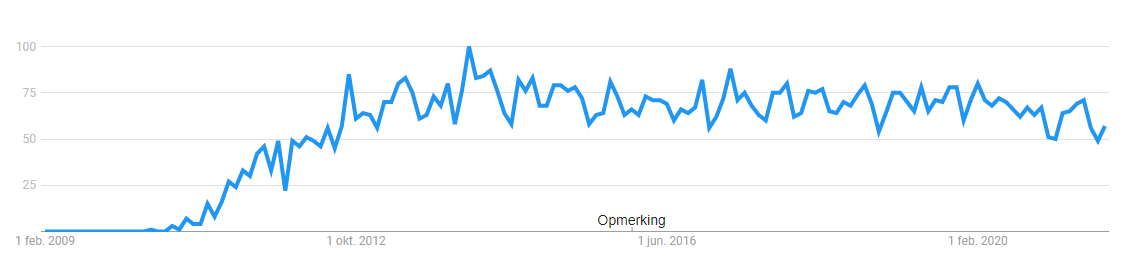
\includegraphics[width=\linewidth]{GoogleTrends.png}
    \caption{Populariteit van gamification \autocite{GoogleTrends2021}.}
    \label{fig:googletrends}
\end{figure}

Bunchball\footnote{https://www.biworldwide.com/gamification/bunchball-nitro/} wordt gezien als het bedrijf dat de gamification-industrie lanceerde. Hun product, Bunchball Nitro, was het eerste technologische platform dat gamemechanismen integreerde in digitale, niet-gaming ervaringen. Sindsdien zijn er tal van toepassingen ontwikkeld binnen verschillende domeinen zoals productiviteit, financiën, gezondheid, onderwijs, duurzaamheid, nieuws en entertainment media \autocite{Groh2012}.

\section{Definitie}

Gamification wordt gebruikt om twee verschillende soorten van ontwikkelingen te beschrijven, \textit{intentional gamification} en \textit{emergent gamification}.

\textit{Intentional gamification} of doelbewuste gamification is een eerste ontwikkeling die volgens \textcite{Deterding2011} wordt beschreven als het gebruik van elementen uit game-design in een niet-gaming context. Het is een opzettelijk proces waarbij een soortgelijke ervaring als in games wordt gecreëerd door activeiten, systemen, diensten of producten om te vormen of te verbeteren. Dit heeft als doel om veranderingen in het gedrag van de gebruiker teweeg te brengen.

\textit{Emergent gamification} of opkomende gamification is een tweede ontwikkeling die dan weer kan worden gedefinieerd als een opkomende, geleidelijke transformatie van cultuur en samenleving die het gevolg is van de steeds groeiende invloed van games. Er wordt verondersteld dat, door de steeds grotere rol van games in het leven van mensen, culturele en maatschappelijke praktijken geleidelijk veranderen in praktijken die kenmerkend zijn aan games, gaminggemeenschappen en spelerspraktijken  \autocite{Hamari2019}.

Zoals eerder werd vermeld, wordt gamification gedefinieerd als het gebruik van elementen uit game-design in een niet-gaming context. Mogelijke doelstellingen worden hierbij uitdrukkelijk weggelaten, dit om de definitie niet onnodig te gaan beperken. In plaats daarvan baseert het zich op de volgende semantische componenten: (1) \textit{game}, (2) \textit{elementen}, (3) \textit{ontwerp} en (4) \textit{niet-gaming context} \autocite{Sailer2016}.

\begin{enumerate}[label=(\arabic*)]
    \item Allereerst moet een onderscheid gemaakt worden tussen \textit{game} of spel en \textit{play} of spelen. Play wordt opgevat als een brede categorie die games omvat maar er van verschilt. \textcite{Caillois2001} verwijst naar het verschil tussen deze twee termen in zijn concept van \textit{paidia} en \textit{ludus}, twee polen van spelactiviteiten. \textit{Paidia} beschrijft vrije, expressieve, improviserende houdingen en betekenissen terwijl \textit{ludus} gekenmerkt is door op regels gebaseerde spellen met vastgelegde doelen. Gamification focust zich zo goed als exclusief op \textit{ludus} met slechts een kleine ruimte voor \textit{paidia}. Gamification heeft dus met andere woorden te maken met de op regels gebaseerde, doelgerichte aard van games \autocite{Sailer2016}.
    \item \textit{Elementen} laten toe om gamification te gaan onderscheiden van ``serieuze games''. In tegenstelling tot ``serieuze games'', omschreven als volwaardige games voor specifieke, niet-entertainment doeleinden, verwijst gamification naar het gebruik van verschillende bouwstenen van games die zijn geïntegreerd in reële contexten \autocite{Groh2012}. \textcite{Deterding20112} stellen voor om game-design elementen te gaan definiëren als elementen die kenmerkend zijn voor games, die voorkomen in de meeste (maar niet noodzakelijk alle) games en een belangrijke rol spelen in de werking en betekenis van de game.
    \item De term \textit{ontwerp} stelt game-design tegenover game-gebaseerde technologieën. De definitie van gamification heeft specifiek betrekking op een doelbewust ontwerpproces terwijl game-gebaseerde technologieën betrekking hebben op facetten zoals game-engines of controllers \autocite{Sailer2016}.
    \item Binnen de \textit{niet-gaming context} wordt er niet nader op ingegaan op de mogelijke gebieden waarin gamification kan worden toegepast, zodat de gebruikscontexten, -doeleinden of -scenario's niet worden afgebakend \autocite{Sailer2016}. De enige context die is uitgesloten, is gamification van games zelf. Dit omdat het een extensie zou zijn van een game zelf en dus als gevolg een deel is van game-design en niet van gamification \autocite{Groh2012}.
\end{enumerate}

\section{De vijf niveaus van game-design}

\textcite{Deterding20112} hebben in hun zoektocht doorheen de bestaande literatuur over games en gamification vijf game-design elementen geïdentificeerd bestaande uit verschillende abstractieniveaus. In Figuur \ref{fig:table1} worden ze gesorteerd op hun abstractieniveau, met bovenaan de meest concrete en onderaan de meeste abstracte.

\begin{figure}
    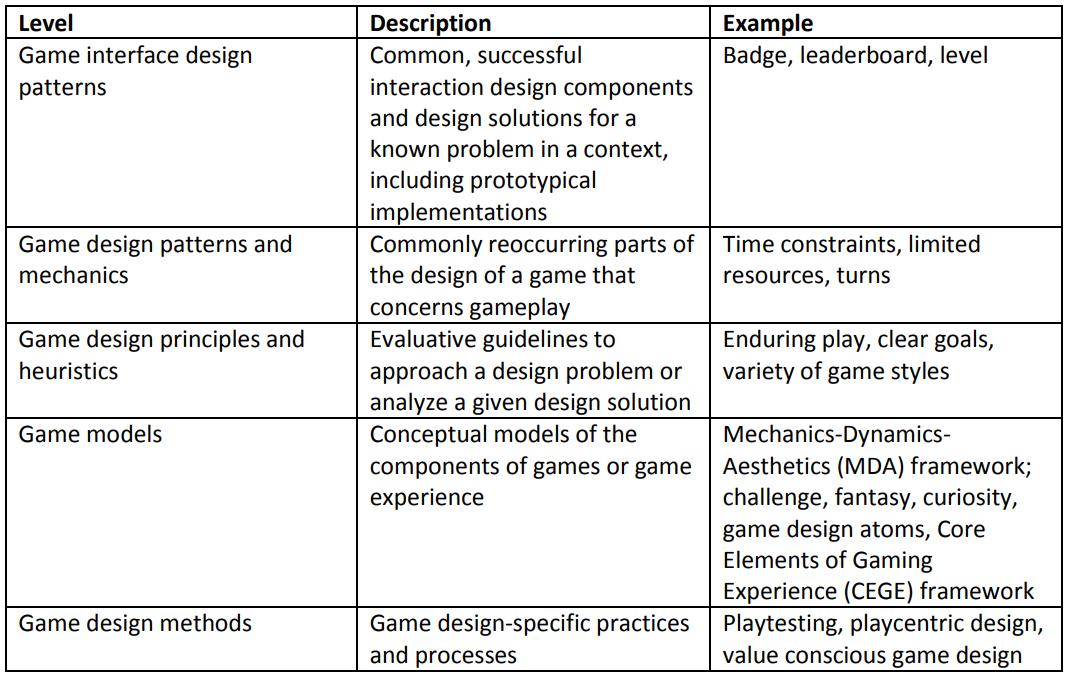
\includegraphics[width=\linewidth]{Deterding2011Table.png}
    \caption{Game-design elementen \autocite{Deterding20112}.}
    \label{fig:table1}
\end{figure}

\subsection{Game-interface ontwerppatronen}

De eerste categorie bevat veelvoorkomende, succesvolle interactie-ontwerpcomponenten, ontwerpoplossingen voor een gekend probleem binnen een bepaalde context en implementaties van prototypes. Badges, leaderboards en levels zijn een aantal voorbeelden van dit game-design element. Het zijn visuele indicatoren die prestaties van gebruikers weergeven \autocite{Morford2014}. Game-interface ontwerppatronen zijn dus met andere woorden elementen die betrekking hebben op wat er getoond gaat worden op het scherm van de gebruiker \autocite{Lindholm2016}.

\subsection{Game-designpatronen en -mechanismen}

Het tweede element wordt beschreven als vaak terugkerende onderdelen van het design van een game die te maken hebben met de gameplay. Deze onderdelen zijn iets wat gebruikers ervaren. Voorbeelden van deze game-designpatronen en -mechanismen zijn tijdsbeperkingen, beurten en beperkte middelen \autocite{Lindholm2016}. \textcite{Morford2014} beschrijven dit element als eigenschappen van een game waarmee gebruikers direct mee omgaan.

\subsection{Game-designprincipes en -heuristieken}

Het derde game-design element gaat over beoordelingsrichtlijnen om een ontwerpprobleem te gaan benaderen of een gegeven ontwerpoplossing te gaan analyseren. Langdurig spelen, duidelijke doelen en een verscheidenheid aan speelstijlen zijn een aantal voorbeelden die de game-designprincipes en -heuristieken karakteriseren.

\subsection{Gamemodellen}

Het vierde niveau heeft betrekking op conceptuele modellen van de componenten van games of game-evervaring. Een aantal van de voorbeelden die eigen zijn aan dit niveau zijn uitdaging, fantasie en nieuwsgierigheid. Het niveau van gamemodellen gaat met andere woorden over conceptuele benaderingen voor het begrijpen van de spelerservaring \autocite{Lindholm2016}.

\subsection{Game-designmethoden}

Ten slotte heeft het vijfde en laatste element te maken met specifieke game-design praktijken en processen ofwel game-design strategieën. Voorbeelden hiervan zijn playtesting, spelgericht ontwerpen en waardebewust game-design.

\section{Vaak voorkomende elementen}

Hieronder worden een aantal van de meest voorkomende en meest besproken game-design elementen meer in detail bekeken. Deze elementen worden nader bekeken door hun directe zichtbaarheid voor de spelers, doordat ze gemakkelijk geactiveerd of gedeactiveerd kunnen worden en omdat ze spelers sterk kunnen motiveren. Ze worden gemakkelijk geïmplementeerd door spelontwerpers omdat ze deel uitmaken van het zichtbare gedeelte van een game en niet van afhankelijk zijn van onderliggende mechanismen \autocite{Sailer2016}.

\subsection{Punten}

Punten zijn een van de elementen die aan de grondslag liggen van een groot aantal toepassingen die gamification implementeren en zijn hierdoor een basisvereiste \autocite{Sailer2016}. Ze zijn de gemakkelijkste manier om een speler te gaan belonen voor de succesvolle voltooiing van een actie, opdracht of een reeks van stappen en om hun vooruitgang in cijfervorm uit te drukken. Deze techniek is nuttig om mensen te gaan motiveren die graag een gevoel van vooruitgang hebben en om mensen aan te moedigen om acties te ondernemen \autocite{Costa2019}.

Voor de ontwerper zijn de punten ook belangrijk want ze houden de acties van alle spelers bij. Op deze manier kan gezien worden hoe spelers omgaan met het systeem, kan het systeem ontworpen worden voor bepaalde resultaten te behalen en kunnen de juiste aanpassingen aan het systeem gedaan worden \autocite{Zichermann2011}.

Het aantal punten dat wordt toegewezen aan een bepaalde actie moet zorgvuldig worden gekozen. Het is imperatief dat de punten afhankelijk zijn van de moeilijkheidsgraad van een taak of actie. Als een speler veel moeilijkheid ondervindt tijdens het uitvoeren van een taak en hiervoor minder punten krijgt zal hij/zij ontmoedigd geraken. Aan de andere kant, als een speler meer punten krijgt voor een makkelijke opdracht zal hij/zij gedemotiveerd geraken \autocite{Costa2019}.

\begin{figure}
    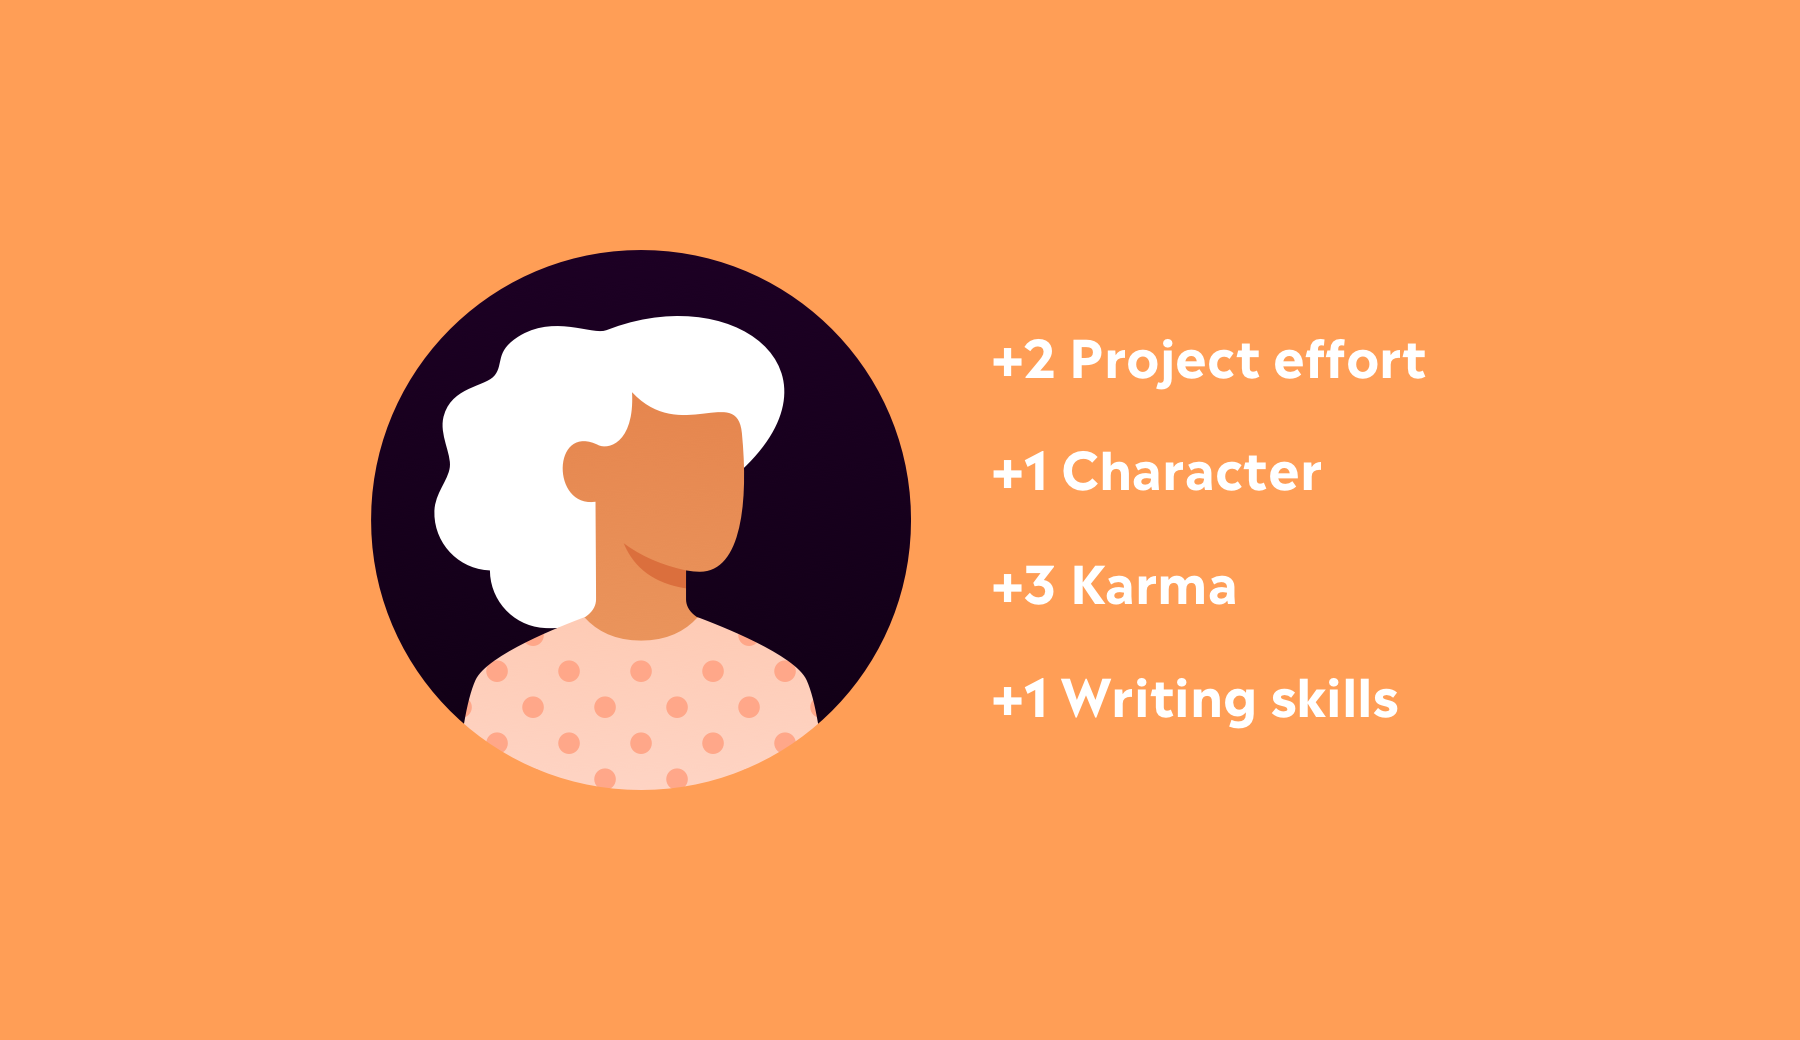
\includegraphics[width=\linewidth]{Points.png}
    \caption{Ervaringspunten \autocite{Points2018}.}
    \label{fig:points}
\end{figure}

Puntensystemen bestaan in alle soorten en maten, van overduidelijk tot nauwelijks zichtbaar \autocite{Zichermann2011}. Een aantal voorbeelden van deze systemen zijn ervaringspunten (weergegeven in Figuur \ref{fig:points}), inwisselbare punten of reputatiepunten \autocite{Sailer2016}. Ook kunnen de punten gerelateerd worden aan andere systemen, zoals leaderboards of niveaus \autocite{Costa2019}.

\subsection{Badges}

Badges worden gedefinieerd als een visuele voorstelling van prestaties of vaardigheden \autocite{Costa2019}. Ze kunnen zowel verdiend als verzameld worden. Het verdienen van een badge kan afhankelijk zijn van bijvoorbeeld een bepaald aantal punten te verzamelen of, zoals weergegeven in Figuur \ref{fig:badges}, een bepaalde activiteit uit te voeren \autocite{Sailer2016}.

\begin{figure}
    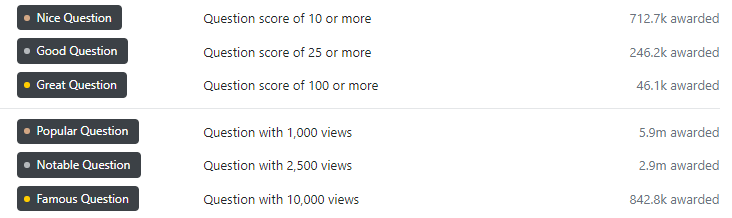
\includegraphics[width=\linewidth]{Badges.png}
    \caption{Badges met hun vereiste acties \autocite{Badges2021}.}
    \label{fig:badges}
\end{figure}

Een badge kan voorkomen in twee verschillende soorten, de zichtbare badges en onzichtbare badges. Een badge is zichtbaar als een speler weet welke actie hij/zij moet ondernemen of welk doel hij/zij moet bereiken. Een onzichtbare badge is een verrassing en wordt op een natuurlijke manier verdiend \autocite{Costa2019}.

Badges kunnen gebruikt worden als referentiesysteem dat de prestaties van spelers bevestigt, hun verdiensten symboliseert, zichtbaar aantoont dat spelers een niveau of doel hebben bereikt \autocite{Anderson2013} en de voortgang van het spel binnen het systeem weergeeft \autocite{Zichermann2011}. Ook kunnen ze fungeren als stimulans, doordat een gebruiker bepaalde acties zal ondernemen om een badge te behalen. Hierdoor wordt het gedrag van gebruikers in een gewenste richting gestuurd. Ten slotte kunnen badges ook dienen als statussymbool, vooral als ze zeldzaam zijn of moeilijk te verdienen \autocite{Sailer2016}. Dit kan opnieuw spelers beïnvloeden om dezelfde acties of stappen te ondernemen om dezelfde badges te verdienen.

\subsection{Scoreborden}

Scoreborden geven een overzicht van deelnemers aan een competitie \autocite{Costa2013} en rangschikken hen volgens hun relatieve succes. Standaard wordt een geordende lijst weergegeven met een score naast elke naam \autocite{Zichermann2011}. Deze score wordt bepaald aan de hand van een succescriterium \autocite{Sailer2016}. Dit succescriterium kan bijvoorbeeld het aantal verzamelde punten zijn.

Een scorebord helpt om te bepalen wie het beste presteert door de prestaties van spelers voor anderen zichtbaar te maken \autocite{Costa2019}. Doordat spelers een eenvoudige vergelijking kunnen maken tussen hun eigen prestaties en die van anderen \autocite{Zichermann2011} kan de competitie tussen spelers in stand gehouden worden. Als dit in de juiste situatie wordt gebruikt kan een scorebord een krachtige motivator zijn \autocite{Costa2019}. Echter kunnen ze ook fungeren als demotivator als spelers zich aan de onderkant van het leaderboard bevinden \autocite{Sailer2016}.

\begin{figure}
    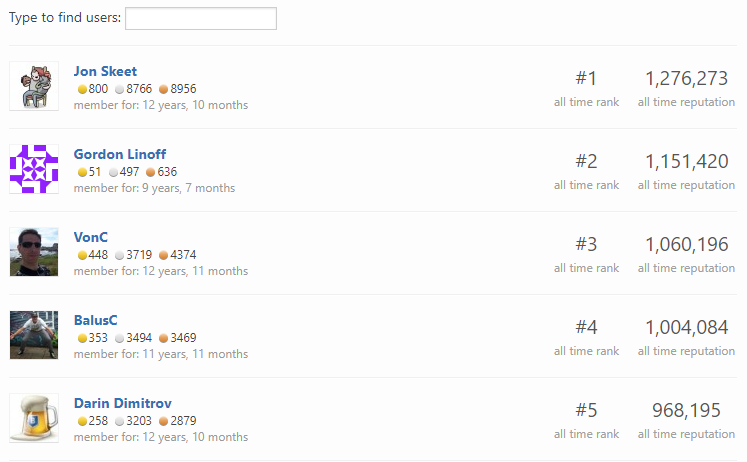
\includegraphics[width=\linewidth]{Leaderboard.png}
    \caption{Reputatiepunten van de top vijf gebruikers \autocite{Leaderboard2021}.}
    \label{fig:leaderboard}
\end{figure}

Er zijn verschillende manieren om een scorebord te ontwerpen. Een ontwerper kan ervoor kiezen om slechts een bepaald deel weer te geven, om geen competitief gedrag aan te moedigen. Dit kan bijvoorbeeld door slechts twee personen boven en onder een speler weer te geven, om hij/zij aan te motiveren. Zoals in Figuur \ref{fig:leaderboard} wordt getoond, kan de ontwerper beslissen om de competitie te vergroten door enkel de top vijf van alle spelers te tonen, waardoor spelers worden aangemoedigd hun score te vergroten \autocite{Costa2019}.

\subsection{Prestatiegrafieken}

Prestatiegrafieken geven informatie weer over de prestaties van een speler in vergelijking met zijn/haar eerdere prestaties \autocite{Sailer2013}. Ze geven dus in tegenstelling tot scoreborden, waar de prestaties van een speler worden vergeleken met die van andere spelers, een evaluatie van de verwezenlijkingen van een speler over een bepaalde periode \autocite{Sailer2016}.
 
Door de prestaties grafisch weer te geven over een bepaalde periode krijgt de speler feedback over zijn/haar verwezenlijkingen, waardoor wordt aangemoedigd om de focus te leggen op verbetering \autocite{Sailer2013}.

\subsection{Betekenisvolle verhalen}

Een betekenisvol verhaal is een ontwerpelement dat niet direct gerelateerd is aan de prestaties van een speler \autocite{Sailer2016}. Binnen platformen die gamification implementeren kunnen, door het toevoegen van een verhaal, activiteiten en opdrachten binnen een bepaalde context worden geplaatst. Ze krijgen hierdoor een betekenis die verder gaat dan louter een zoektocht naar punten en prestaties \autocite{Kapp2012}.

Door een betekenis te geven aan activiteiten en opdrachten krijgen spelers een gevoel van inspiratie en motivatie, vooral als het verhaal aansluit bij hun persoonlijke interesses \autocite{Sailer2016}. Verhalen kunnen ook positieve gevoelens opwekken en versterken \autocite{Sailer2013}.

\subsection{Avatars}

Avatars zijn een visuele representatie van de speler binnen de gamification omgeving \autocite{Sailer2016}. De avatar wordt meestal zelf gekozen of gecreërd \autocite{Kapp2012}. Ze delen de identiteit, aanwezigheid, locatie, en activiteiten van de speler met anderen \autocite{Annetta2010}.

Een avatar kan een een complexe, geanimeerde driedimensionale representatie zijn \autocite{Sailer2016} maar kan ook eenvoudigweg een kleine pictogram zijn met een gebruikersnaam \autocite{Zichermann2011}. De belangrijkste vereiste is dat ze de spelers identificeren en hen onderscheiden van anderen \autocite{Sailer2016}.

Gelijk welke vorm een avatar aanneemt, ze laten toe dat de speler een andere identiteit kan aannemen en deel kan uitmaken van een gemeenschap \autocite{Annetta2010}. Dit kan spelers een gevoel van autonomie geven en positieve gevoelens geven door een ontwikkelingsproces met de avatar aan te gaan \autocite{Sailer2013}.

\subsection{Teamleden}

Door teams te introduceren, gedefinieerd als afgebakende groepen van spelers die samenwerken aan een doel, kan samenwerking worden bevorderd \autocite{Sailer2016}. Tussen de verschillende teamleden kan echter ook een rivaliteit tot stand komen of kunnen conflicten ontstaan \autocite{Kapp2012}.

\section{Gedrag beïnvloeden}

Een van de belangrijkste doelen van gamification is het gedrag van een gebruiker beïnvloeden \autocite{AlMarshedi2015}. Volgens het gedragsmodel van \textcite{Fogg2009} moet een persoon of gebruiker eerst een bepaald niveau van motivatie bereiken en de mogelijkheid krijgen om het gedrag te vertonen. Zodra deze twee toestanden zijn bereikt is enkel nog een trigger nodig om het gewenste gedrag tevoorschijn te laten komen.

\subsection{Motivatie}

Motivatie is het verlangen om iets te doen. Het is belangrijk om hiermee rekening te houden bij gamification, in het bijzonder omdat het gedrag van mensen stuurt \autocite{AlMarshedi2015}. In het algemeen bestaan twee soorten van menselijk motivatie: (1) \textit{intrinsieke motivatie} en (2) \textit{extrinsieke motivatie} \autocite{Yang2017}.

\begin{enumerate}[label=(\arabic*)]
    \item \textit{Intrinsieke motivatie} wordt gedefinieerd als een intern verlangen om dingen te doen uit plezier of liefde \autocite{AlMarshedi2015}, ofwel een activiteit nastreven omdat deze inherent interessant of plezierig is. Wanneer een persoon intrinsiek gemotiveerd is, zal hij/zij dus bewogen worden om te handelen voor het plezier of de uitdaging in plaats van te bewogen te worden vanwege beloningen of externe druk. Het is een natuurlijke aanleg voor ontdekking, bekwaamheid en spontane interesse dat de volharding, prestaties en het welzijn ten goede komen \autocite{Dahlstrom2018}. 
    \item \textit{Extrinsieke motivatie} kan worden beschreven als dingen doen uitsluitend voor het resultaat \autocite{AlMarshedi2015}. Het wordt vaak geassocieerd met voornamelijk de wens om beloningen te krijgen en bestraffing te vermijden, wat wordt gezien als minder ideaal voor het welzijn van mensen dan intrinsieke motivatie. Extrinsieke motivatie kan sterk variëren in welke vorm deze voorkomt en kan toch leiden tot een grotere ervaring van welzijn, afhankelijk  van hoeveel gevoel van autonomie deze de persoon in kwestie geeft \autocite{Dahlstrom2018}.
\end{enumerate}

Een groot aantal gamificationtoepassingen en -diensten richten zich tegenwoordig op motivatie, vooral van het extrinsieke type. Extrinsieke motivatie kan echter niet als enige manier gebruikt worden om gedrag te veranderen. Dit komt omdat extrinsieke motivatie sterk afhangt van individuele kenmerken. De gedragsverandering kan dus van tijdelijke aard zijn en zorgt dus niet voor een duurzaam effect. Een goed inzicht krijgen in de verschillende soorten van motivatie en hoe gedrag tot stand komt is dus van cruciaal belang bij het ontwerpen van toepassingen en diensten die gamification implementeren \autocite{AlMarshedi2015}.

\section{Hexad Framework}

De ``Big Five'' persoonlijkheidsfactoren, een beschrijvend model van persoonlijkheid, is in het verleden al uitgebreid gebruikt geweest om de psychologie achter gebruikersmotivatie te onderzoeken \autocite{Yuan2016}. Dit model schiet echter tekort omdat het niet specifiek bedoeld is voor gamification.

Om een beter inzicht te krijgen in wat de gebruiker motiveert en om de ervaring te personaliseren binnen een omgeving die gamification implementeerd, hebben \textcite{Tondello2016} het Hexad Framework ontwikkeld. Het is specifiek ontworpen naar gebruikersmotivatie binnen gamification en het dient om zes gebruikerstypes te linken aan verschillende ontwerpelementen.

\subsection{Gebruikerstypes}

\textcite{Marczewski2015} stelde zes gebruikerstypes voor, zichtbaar in Figuur \ref{fig:usertypes}, die verschillen in de mate waarin ze gemotiveerd kunnen worden door intrinsieke of extrinsieke motiverende factoren, namelijk (1) \textit{filantropen}, (2) \textit{socialisers}, (3) \textit{vrije geesten}, (4) \textit{presteerders}, (5) \textit{spelers} en (6) \textit{ontwrichters}.

\begin{enumerate}[label=(\arabic*)]
    \item \textit{Filantropen} zijn altruïstisch en zijn bereid om te geven zonder een beloning te verwachten. Ze worden gemotiveerd door een doel. Enkele van de voorgestelde ontwerpelementen voor filantropen zijn: verzamelen en handelen, schenken, delen van kennis en administratieve rollen.
    \item \textit{Socialisers} willen met anderen omgaan en social banden scheppen. Ze worden gemotiveerd door verwantschap. Ontwerpelementen die socialisers motiveren zijn teams, sociale netwerken, social vergelijking, sociale competitie en sociale ontdekking.
    \item \textit{Vrije geesten} worden gemotiveerd door autonomie, meer bepaald vrijheid om zichzelf te uiten en te handelen zonder controle van buitenaf. Ze willen vooral creëren en verkennen binnen een systeem. De ontwerpelementen die het beste bij hun passen zijn: verkennende taken, tools voor creativiteit, ontgrendelbare content, niet-lineaire gameplay en Easter eggs.
    \item Competentie is de sterkste motivator voor \textit{presteerders}. Ze proberen vooruit te geraken binnen een systeem door taken te voltooien of moeilijke uitdagingen aan te gaan. Uitdagingen, certificaten, het leren van nieuwe vaardigheden, niveaus en progressie zijn enkele van de elementen die bij hun passen.
    \item \textit{Spelers} zullen er alles aan doen om een beloning te verdienen binnen een systeem, ongeacht het type activiteit. Ze worden het meeste gemotiveerd door extrinsieke beloningen. Ontwerpelementen waarvoor spelers de voorkeur hebben zijn punten, scoreborden, badges, beloningen of prijzen en virtuele economieën.
    \item \textit{Ontwrichters} willen verandering teweegbrengen. Ze willen het systeem ontwrichten, op zowel een positieve als negatieve manier, om veranderingen af te dwingen. Ze houden ervan om de grenzen van het systeem af te tasten en deze grenzen steeds verder te verleggen. Enkele voorgestelde ontwerpelementen zijn: innovatieplatformen, ontwerptools, anonimiteit en anarchistische gameplay.
\end{enumerate}

Het is belangrijk om op te merken dat individuen zelden binnen één bepaald type passen. Gebruikers zullen vaak een een hoofdtendens vertonen maar ze zullen in de meeste gevallen ook tot op zekere hoogte binnen andere types passen \autocite{Tondello2016}.

\begin{figure}
    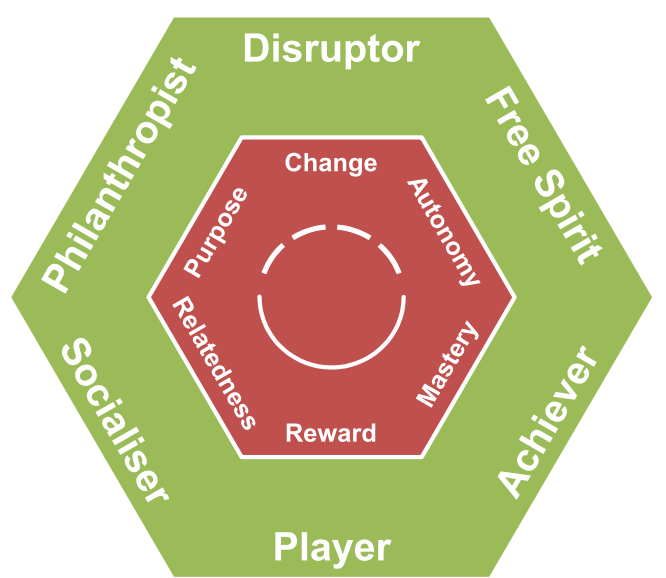
\includegraphics[width=\linewidth]{HexadUserTypes.png}
    \caption{De Hexad gebruikerstypes \autocite{Tondello2016}.}
    \label{fig:usertypes}
\end{figure}

\subsection{Methodologie}



Via de voorgestelde enquête en data-analyse kunnen ontwerpers hun doelpubliek screenen en de juiste ontwerpelementen kiezen, gepersonaliseerd voor elke gebruiker. Binnen onderzoek kunnen de resultaten gebruikt worden om een beter begrip te krijgen over de betrokkenheid van gebruikers en hun plezier van gebruik \autocite{Tondello2016}.



%%=============================================================================
%% Methodologie
%%=============================================================================

\chapter{\IfLanguageName{dutch}{Methodologie}{Methodology}}
\label{ch:methodologie}

%% TODO: Hoe ben je te werk gegaan? Verdeel je onderzoek in grote fasen, en
%% licht in elke fase toe welke stappen je gevolgd hebt. Verantwoord waarom je
%% op deze manier te werk gegaan bent. Je moet kunnen aantonen dat je de best
%% mogelijke manier toegepast hebt om een antwoord te vinden op de
%% onderzoeksvraag.


%%=============================================================================
%% Prototype
%%=============================================================================

\chapter{Prototype}
\label{ch:prototype}

\section{Inleiding}

In dit hoofdstuk zullen een aantal van de verschillende ontwerpelementen, die zijn toegelicht in de literatuurstudie, worden toegevoegd aan het bestaande platform Innerdreams, met als doel gamification te implementeren. De keuze werd gemaakt om gebruikers toe te laten punten en badges te verzamelen en om een scorebord en beloningswinkel toe te voegen. Deze elementen werden gekozen na een brainstormsessie en een kort onderzoek over de verschillende manieren waarop gamification kan worden geïmplementeerd.

\section{Requirements}

Zoals in de inleiding werd vermeld werd gekozen om een puntensysteem te implementeren.  Gebruikers moeten punten kunnen verzamelen door enquêtes in te vullen en te delen. Meer specifiek moet een gebruiker punten kunnen verzamelen per volledig succesvol ingevulde pagina van een enquête en als een enquête volledig wordt voltooid. Punten moeten ook kunnen worden verzameld als een gebruiker de afgelegde enquête deelt en als deze gedeelde enquête succesvol wordt voltooid door de persoon waarmee deze gedeeld werd. Ook moeten gebruikers badges kunnen verzamelen als een mijlpaal wordt bereikt. Hier werd gekozen om het behalen van badges enkel te laten afhangen van het afleggen van enquêtes. Vervolgens moet een gebruiker ook een scorebord kunnen raadplegen waarin de rangschikking, gebruikersnaam en het totaal aantal verzamelde punten van alle gebruikers zal worden weergegeven. Ten slotte moet het mogelijk zijn voor een gebruiker om zijn/haar verzamelde punten te gebruiken in een beloningswinkel om verschillende artikelen aan te schaffen.

\section{Uitwerking}

\subsection{Puntensysteem}

Om het puntensysteem uit te werken werd gekozen om gebruikers punten te laten verzamelen bij het invullen en delen van enquêtes. Hiervoor is het nodig dat de mogelijkheid bestaat om aan bepaalde enquêtes punten te gaan toewijzen.

Een eerste noodzakelijke aanpassing was het toevoegen van een tabel aan de SQL databank om de punten die kunnen toegewezen worden aan de verschillende onderdelen van een enquête bij te houden. Zoals te zien is in Figuur \ref{fig:dbdiagram} bestaat de tabel uit de volgende kolommen:

\begin{itemize}
    \item PuntenID: de primaire sleutel om de punten te identificeren.
    \item Pagina: het aantal punten dat wordt verdiend bij het volledig invullen van een pagina van een enquête.
    \item EnqueteCompleted: het aantal punten dat wordt verdiend bij het volledig voltooien van een enquête.
    \item Share: het aantal punten dat wordt verdiend bij het delen van een enquête.
    \item ShareCompleted: het aantal punten dat wordt verdiend bij het succesvol voltooien van een enquête door de persoon met wie de enquête is gedeeld.
    \item EnqueteID: de vreemde sleutel die de punten linkt aan een enquête.
\end{itemize}

\begin{figure}
    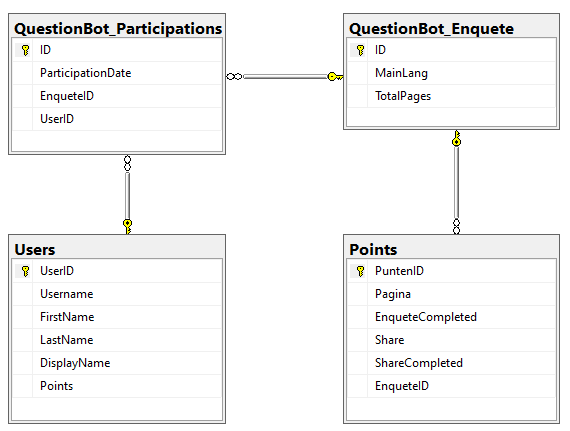
\includegraphics[width=\linewidth]{DBDiagram.png}
    \caption{Het model van de punten.}
    \label{fig:dbdiagram}
\end{figure}

Het was ook nodig om het totale aantal verzamelde punten van iedere individuele gebruiker bij te houden. In Figuur \ref{fig:dbdiagram} is te zien dat aan de gebruikerstabel een extra kolom werd toegevoegd om deze punten vast te hangen aan de gebruikers. Voor zowel gebruikers die een nieuw profiel aanmaken als voor de reeds bestaande gebruikers werd de standaard waarde van hun punten op nul gezet.

Eenmaal een gebruiker het einde van een enquête bereikt is het nodig om een overzicht van het totale aantal verzamelde punten tijdens het afleggen van de enquête weer te geven. Het is daarom dat werd gekozen om ook een overzichtspagina toe te voegen. Deze pagina verschijnt eenmaal een gebruiker een enquête volledig heeft ingevuld en de inhoud hiervan hangt af van of een enquête punten heeft toegewezen gekregen of niet. Als de enquête punten heeft toegewezen gekregen zal op deze pagina een overzicht worden getoond van de verzamelde punten tijdens het afleggen van de enquête. Op deze pagina is het ook mogelijk om de enquête te gaan delen met andere gebruikers, waardoor nog meer punten kunnen worden verdiend. Als de enquête geen punten heeft toegewezen gekregen zal op dit overzicht een korte bedanking worden getoond.

Soms is het ook mogelijk dat een gebruiker niet moet aangemeld zijn om een enquête in te vullen. Om te zorgen dat de punten die de gebruiker heeft verzameld niet verloren gaan worden deze bijgehouden in zogenaamde sessievariabelen. Een sessievariabele is een object dat voor elke gebruiker apart wordt bijgehouden op de server zolang een sessie tussen de gebruiker en de server actief is. De totale waarde van de verzamelde punten wordt bijgehouden in een sessievariabele tijdens het afleggen van een enquête. Eenmaal de gebruiker op de overzichtspagina terechtkomt en niet aangemeld is wordt de optie gegeven om zich alsnog aan te melden. Als de gebruiker na de doorverwijzing naar de aanmeldpagina terug wordt doorverwezen naar de overzichtspagina zal hij/zij een overzicht zien van de verzamelde punten die bijgehouden zijn in de sessievariabele. Hier krijgt de gebruiker alsnog de kans om de punten te verzilveren.

Als een gebruiker kiest om een enquête te delen zal de URL van de gedeelde enquête een aantal extra parameters bevatten. Een van deze parameters bevat een uniek cijfer dat de gebruiker die de enquête heeft gedeeld zal identificeren. Bij de start van het afleggen van een enquête wordt een controle uitgevoerd om de URL. Als deze URL de eerder vermelde unieke identificatie bevat zullen aan deze gebruiker een aantal vooraf bepaalde punten worden toegewezen. Eenmaal de enquête wordt voltooid zullen aan deze gebruiker opnieuw een aantal punten worden toegewezen.

\subsection{Badgesysteem}

Voor het behalen van badges werd gekozen om deze te gaan koppelen aan het totale aantal deelnames van een gebruiker aan enquêtes. Een deelname wordt toegevoegd aan de databank eenmaal een gebruiker tenminste één pagina heeft ingevuld van een enquête.

In figuur \ref{fig:dbbadge} is te zien dat voor het bijhouden van de verschillende badges een extra tabel werd toegevoegd aan de SQL databank. Deze tabel bestaat uit de volgende kolommen:

\begin{itemize}
    \item ID: de primaire sleutel om de badge te identificeren.
    \item ImageLink: een verwijzing naar de afbeelding van de badge.
    \item Title: een titel die de badge beschrijft.
    \item TriggerQuery: een SQL-query die wordt uitgevoerd eenmaal aan een bepaalde voorwaarde voldaan is.
\end{itemize}

\begin{figure}
    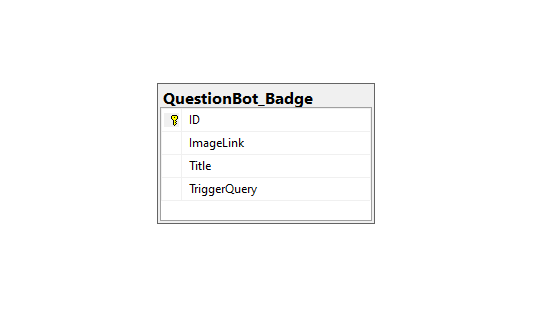
\includegraphics[width=\linewidth]{DBBadge2.png}
    \caption{De badge tabel.}
    \label{fig:dbbadge}
\end{figure}

Wanneer de gebruiker de enquête volledig heeft ingevuld en op de overzichtspagina terechtkomt zullen twee lijsten van badges worden opgehaald. De eerste lijst van badges bestaat uit alle badges die op dat moment aan het systeem zijn toegevoegd. De tweede lijst van badges omvat alle badges die een gebruiker heeft behaald tijdens het invullen van enquêtes. Eenmaal deze twee lijsten zijn opgehaald zullen deze met elkaar worden vergeleken op basis van de unieke identificatie van de badges. Eenmaal een badge wordt tegengekomen die de gebruiker nog niet heeft behaald zal worden gecontroleerd of hij/zij voldoet aan de voorwaarden om deze te behalen. Deze controle zal gebeuren aan de hand van het uitvoeren van een stored procedure, die te zien is in Listing \ref{lst:csb}. In deze stored procedure zal de eerder vermelde trigger query, die gelinkt is aan de desbetreffende badge, worden uitgevoerd.

\begin{lstlisting}[caption={De CheckSucceededBadge stored procedure.},
    label={lst:csb},
    language=SQL,
    showspaces=false,
    basicstyle=\ttfamily,
    numbers=left,
    numberstyle=\tiny,
    numbersep=1pt,
    breaklines=true
    commentstyle=\color{gray}]
    ALTER PROCEDURE [dbo].[QuestionBot_CheckSucceededBadge](@BadgeID int, @UserID int) as
    BEGIN
    Declare @statement as nvarchar(max) 
    set @statement = (select TriggerQuery from QuestionBot_Badge where ID = @BadgeID) 
    EXECUTE sp_executesql @statement , N'@UserID int',@UserID=@UserID
    END
\end{lstlisting}

In Listing \ref{lst:tq} is te zien hoe zo een trigger query eruitziet en functioneert. Voor een specifieke gebruiker wordt de som van het totale aantal deelnames aan alle enquêtes genomen. Als deze som voldoet aan een bepaalde voorwaarde zal een bit geretourneerd worden. Als deze bit 1 is wil dit zeggen dat de gebruiker aan de voorwaarde voldoet en dat de badge behaald is. Als deze bit op 0 staat is niet aan de voorwaarde voldaan en zal de gebruiker de badge niet krijgen. In dit voorbeeld is te zien dat voor de huidige gebruiker wordt gecontroleerd of hij/zij minstens één deelname heeft aan een enquête. Als aan deze voorwaarde is voldaan zal deze gebruiker een badge verdienen met bijvoorbeeld de tekst ``Vul je eerste enquête in'' (Figuur \ref{fig:badgeunlocked}).

\begin{figure}
    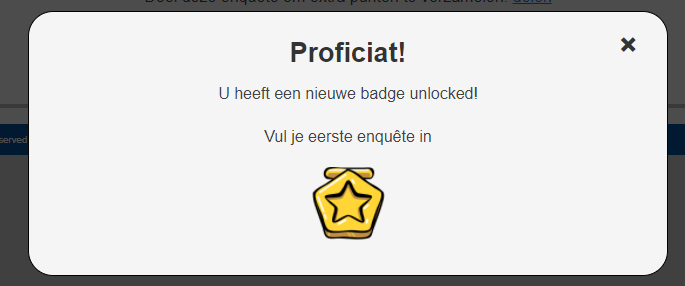
\includegraphics[width=\linewidth]{BadgeUnlocked.png}
    \caption{Het behalen van een badge op Innerdreams.}
    \label{fig:badgeunlocked}
\end{figure}

\begin{lstlisting}[caption={De trigger query van een badge.},
    label={lst:tq},
    language=SQL,
    showspaces=false,
    basicstyle=\ttfamily,
    numbers=left,
    numberstyle=\tiny,
    numbersep=1pt,
    breaklines=true
    commentstyle=\color{gray}]
    declare @Participations int set @Participations = (select count(*) from QuestionBot_Participations where UserID = @UserID) 
    if (@Participations >= 1) select 1 else select 0
\end{lstlisting}

\subsection{Scorebord}

Het scorebord werd ontworpen om respectievelijk de rangschikking, de gebruikersnaam en het totale aantal verzamelde punten van alle gebruikers weer te geven. Om het scorebord te implementeren was het niet nodig om aanpassingen te doen aan de databank. Alle noodzakelijke aanpassingen werden reeds uitgevoerd tijdens het implementeren van de ontwerpelementen in de vorige stappen.

In Listing \ref{lst:gul} is te zien dat gebruik gemaakt werd van een stored procedure, om alle benodigde data van de gebruikers op te halen. In deze stored procedure werd gebruik gemaakt van de \textit{SQL ROW\_NUMBER()} functie. Deze functie zal één of meerdere specifieke kolommen uit een tabel ophalen. Deze kolommen kunnen zowel oplopend als aflopend gesorteerd worden. Na het ophalen zal de functie aan elke rij uit de resultatenlijst een unieke, oplopende waarde toewijzen op basis van de geordende kolom. In dit geval haalt de functie een oplopende lijst van de punten van de gebruikers op en een lijst van de gebruikersnamen. De functie wijst daarna een waarde toe aan elke rij op basis van de puntenlijst. Deze waarde stelt de rangschikking op het scorebord voor. In het geval dat twee gelijke waarden worden tegengekomen in de lijst van punten wijst de functie de waarde toe op basis van de alfabetische volgorde van de gebruikersnamen. Buiten het ophalen van de rangschikking zal deze stored procedure ook de gebruikersnamen en het totale aantal behaalde punten ophalen van alle gebruikers.

\begin{lstlisting}[caption={De GetUsersLeaderboard stored procedure.},
    label={lst:gul},
    language=SQL,
    showspaces=false,
    basicstyle=\ttfamily,
    numbers=left,
    numberstyle=\tiny,
    numbersep=1pt,
    breaklines=true
    commentstyle=\color{gray}]
    ALTER procedure [dbo].[GetUsersLeaderboard] as
    select ROW_NUMBER() OVER(ORDER BY Points desc, DisplayName) as Rank, DisplayName, Points from dbo.Users
    where IsSuperUser = 0
\end{lstlisting}

Eenmaal de data is opgehaald door de stored procedure zal deze in een overzichtelijke tabel worden weergegeven. In Figuur \ref{fig:leaderboardinnerdreams} is het scorebord zoals het binnen Innerdreams is geïmplementeerd te zien. Binnen dit scorebord kan worden gesorteerd en gefilterd. Sorteren kan gebeuren zowel op de rangschikking, de gebruikersnaam als het aantal behaalde punten en filteren kan gebeuren op de gebruikersnaam. Initeel zal het scorebord alle gebruikers weergeven maar de keuze kan ook gemaakt worden om enkel de top vijf van alle gebruikers met het meeste aantal punten weer te geven.

\begin{figure}
    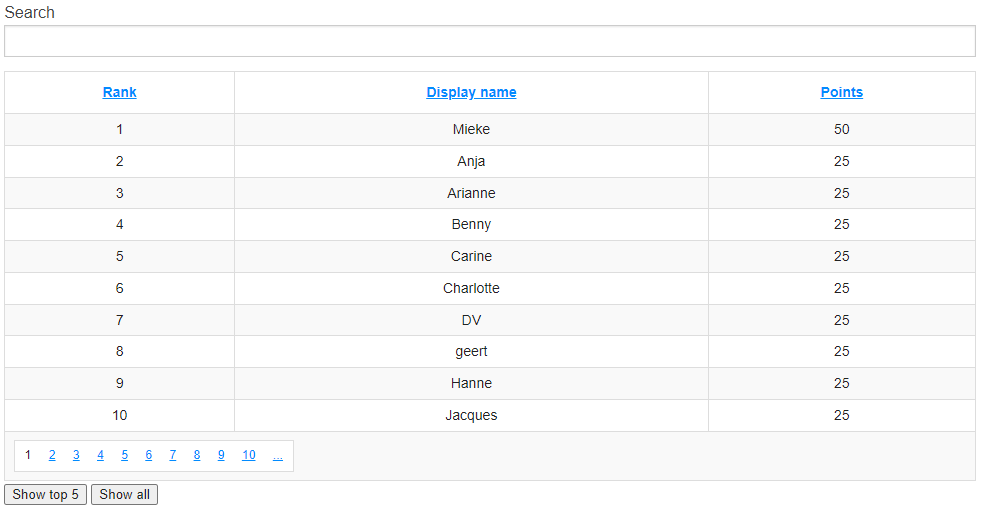
\includegraphics[width=\linewidth]{LeaderboardInnerdreams.png}
    \caption{Het scorebord op Innerdreams.}
    \label{fig:leaderboardinnerdreams}
\end{figure}

\subsection{Beloningswinkel}

Om de punten die de gebruikers hebben verzameld tijdens het afleggen van de verschillende enquêtes niet verloren te laten gaan is het nodig dat deze punten ergens gespendeerd kunnen worden. Het is daarom dat als laatste ontwerpelement werd gekozen om een beloningswinkel te ontwerpen en te gaan implementeren. In deze winkel is het mogelijk om met de verzamelde punten een grote verscheidenheid aan artikelen aan te schaffen.

Om te beginnen met de beloningswinkel te implementeren waren opnieuw een aantal aanpassingen nodig aan de SQL databank. In Figuur \ref{fig:dbdiagramreward} is te zien dat het ten eerste nodig was om een nieuwe tabel toe te voegen waarin de beloningen zelf worden bijgehouden. Deze tabel bestaat uit de volgende kolommen:

\begin{itemize}
    \item RewardID: de primaire sleutel om de beloning te identificeren.
    \item Titel: de titel van de beloning.
    \item Beschrijving: een korte tekst die de beloning beschrijft.
    \item Stock: de hoeveelheid beschikbare beloningen.
    \item Prijs: hoeveel punten nodig zijn om een beloning aan te schaffen.
    \item Startdatum: de datum waarop een beloning actief wordt.
    \item Einddatum: de datum waarop een beloning niet langer actief is.
    \item AantalClaimed: de hoeveelheid beloningen die al aangeschaft zijn.
    \item LeverbaarIn: de landen waarin de beloning beschikbaar is.
    \item ImageLink: een verwijzing naar de afbeelding van de beloning.
    \item AantalPerPersoon: hoeveel beloningen één persoon kan aanschaffen.
    \item VerplichteEnquetes: welke enquêtes verplicht moeten worden voltooid.
    \item Mail: e-mail die wordt verstuurd naar de gebruiker eenmaal een beloning is aangeschaft.
\end{itemize}

\begin{figure}
    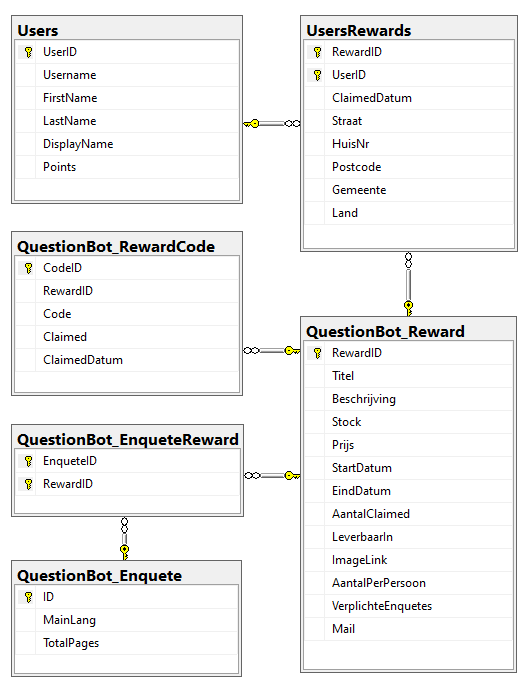
\includegraphics[width=\linewidth]{DBDiagramReward.png}
    \caption{Het model van de beloningen.}
    \label{fig:dbdiagramreward}
\end{figure}

Om een beloning aan te kopen kan ook gebruik gemaakt worden van een beloningscode. De informatie over deze codes wordt bijgehouden in een tabel en hiervoor was het opnieuw nodig om een tabel toe te voegen aan de SQL databank. In Figuur \ref{fig:dbdiagramreward} is de tabel te zien en deze bestaat uit de volgende kolommen:

\begin{itemize}
    \item CodeID: de primaire sleutel om de code te identificeren.
    \item RewardID: de vreemde sleutel die de codes linkt aan een beloning.
    \item Code: de code die gebruikt kan worden om een beloning aan te schaffen.
    \item Claimed: een controle of de code al gebruikt is of niet.
    \item ClaimedDatum: de datum waarop de code is gebruikt.
\end{itemize}

Een beloning zal vaak niet zomaar kunnen worden aangeschaft. Een gebruiker zal één of meerdere enquêtes verplicht moeten voltooien voordat hij/zij in aanmerking komt om de beloning aan te kopen. Het is ook belangrijk om bij te houden waar een beloning beschikbaar is. Dit omdat ze niet altijd beschikbaar zullen zijn in sommige landen.

In Figuur \ref{fig:rewardshop} is te zien hoe de beloningswinkel op Innerdreams eruit ziet. In dit voorbeeld heeft de beloning een kost van 5 punten.

\begin{figure}
    \includegraphics[scale=0.95]{RewardShop.png}
    \centering
    \caption{De beloningswinkel op Innerdreams.}
    \label{fig:rewardshop}
\end{figure}

\section{Bespreking}

Uit het toevoegen van de verschillende ontwerpelementen aan het prototype blijkt dat bijna geen aanpassingen nodig waren aan het bestaande platform. De enige aanpassing die noodzakelijk bleek te zijn was om aan de bestaande gebruikerstabel een extra kolom toe te voegen waarin de verzamelde punten worden bijgehouden. Alle overige benodigde elementen konden ingewerkt worden binnen het bestaande platform zonder de werking van de bestaande functionaliteiten te verstoren.
%%=============================================================================
%% Gebruikersonderzoek
%%=============================================================================

\chapter{Gebruikersonderzoek}
\label{ch:gebruikersonderzoek}

\section{Inleiding}

De enquête werd volledig anoniem afgenomen.


\section{Resultaten en analyse}

In de volgende secties zullen de resultaten van de enquête besproken en geanalyseerd worden.

\subsection{Demografie}

\textbf{Resultaat}

De grootte van de steekproef bedraagt 66 deelnemers. De verdeling van deze deelnemers volgens hun geslacht en leeftijden wordt weergegeven in de Tabellen \ref{tab:verdelinggeslacht} en \ref{tab:verdelingleeftijden}. In tabel \ref{tab:verdelinggeslacht} is te zien dat de steekproef uit iets meer vrouwen (57,6\%) dan mannen (42,4\%) bestaat. Tabel \ref{tab:verdelingleeftijden} toont dat de deelnemers werden onderverdeeld op basis van hun leeftijd in zeven categorieën. Hieruit is op te maken dat de leeftijden varieerden van jonger dan 18 jaar tot ouder dan 65 jaar. Ook is te zien dat 31,8\% van de bevraagden binnen de leeftijdscategorie 26-35 jaar valt.

\begin{table}
\begin{center}
    \begin{tabular}{c|c|c}
        & \textbf{Totaal} & \textbf{Percentage} (\%) \\
        \hline
        Man & 28 & 42,4\% \\
        \hline
        Vrouw & 38 & 57,6\% \\
    \end{tabular}
\end{center}
\caption{Verdeling van de geslachten.}
\label{tab:verdelinggeslacht}
\end{table}

\begin{table}
    \begin{center}
        \begin{tabular}{c|c|c}
            & \textbf{Totaal} & \textbf{Percentage} (\%) \\
            \hline
            <18 jaar & 4 & 6,1\% \\
            \hline
            18-25 jaar & 12 & 18,2\% \\
            \hline
            26-35 jaar & 21 & 31,8\% \\
            \hline
            36-45 jaar & 7 & 10,6\% \\
            \hline
            46-55 jaar & 5 & 7,6\% \\
            \hline
            56-65 jaar & 11 & 16,7\% \\
            \hline
            >65 jaar & 6 & 9,1\% \\
        \end{tabular}
    \end{center}
\caption{Verdeling van de leeftijden.}
\label{tab:verdelingleeftijden}
\end{table}

\textbf{Bespreking}

De grootte van de steekproef (N = 66) is klein met een ongelijke verdeling van de leeftijdscategorieën. In Tabel \ref{tab:verdelingleeftijden} is te zien dat een aantal van de categorieën een aandeel heeft van minder dan 8 deelnemers. Door deze kleine steekproefgrootte en de ongelijke verdeling van de leeftijden kan deze steekproef niet als representatief worden aanzien.

\subsection{Hexad schaal}

Deelnemers werden onderverdeeld aan de hand van de Gamification User Types Hexad Scale of korter gezegd, de Hexad schaal. Deze onderverdeling gebeurde op basis van de 24 vragen die gesteld werden in het tweede deel van de online enquête. Per gebruikerstype werden vier vragen gesteld op een Likert-schaal van 7 punten. Het totaal van de scores behorende bij deze 4 vragen werd opgeteld tot een getal tussen 4 en 28. Zo werd een score bepaald voor elk gebruikerstype. Het maximum van deze scores is het gebruikerstype dat bij die deelnemer past. Per gebruikerstype werd het aantal personen geteld die hierbij de hoogste score behaalde. Soms kwam het voor dat een deelnemer voor meerdere gebruikerstypes een gelijke score behaalde. Als dit voorkwam werd het aantal dat opgeteld werd bij elk gebruikerstype waarvoor de deelnemer een gelijke score heeft berekend door 1 gedeeld door het aantal types. Een deelnemer heeft bijvoorbeeld een gelijke score behaald bij 3 gebruikerstypes. Bij elk type zal het aantal dan verhoogd worden met 0.33.

\textbf{Resultaten}

In figuur \ref{fig:vergelijkingonderzoek} is een vergelijking te zien tussen de verdeling van de steekproef uit het onderzoek van \textcite{Tondello2016} en de verdeling van de steekproef van dit onderzoek. Hierin is te zien dat er een verschil bestaat in de verdeling van de gebruikerstypes. Voor dit onderzoek is een verdeling te zien waarbij Filantropen de grootste groep vormen met 32.0\%, gevolgd door de Socialisers en Presteerders met elk een aandeel van 20.6\%. Daarna komen de Spelers en Vrije geesten met een aandeel van 15.5\% en 11.3\% respectievelijk. Geen enkele van de deelnemers heeft het Ontwrichter gebruikerstype toegewezen kreeg

\begin{figure}
    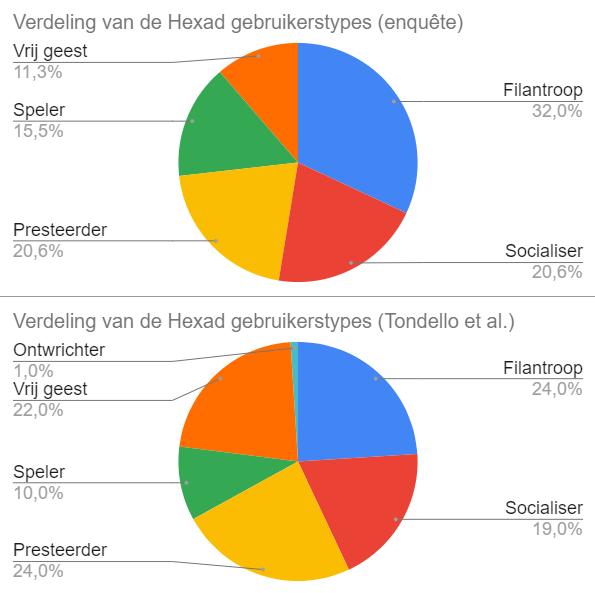
\includegraphics[width=\linewidth]{VergelijkingOnderzoek.png}
    \caption{Vergelijking van de verdeling van de gebruikerstypes.}
    \label{fig:vergelijkingonderzoek}
\end{figure}

De verdeling van de gebruikerstypes per geslacht is te zien in Figuur \ref{fig:verdelinggeslacht}. Hierin is te zien dat een groter aandeel van Filantropen, Socialisers en Presteerders te vinden is bij de vrouwen. Bij de mannen is dan weer een groter aantal Spelers en Vrije geesten te vinden. Via de onafhankelijkheidstoets werd nagegaan of een verband bestaat tussen de gebruikerstypes en het geslacht. In Tabel \ref{tab:onafhankelijkheidstoets} is te zien dat hierbij $\chi^2$(4) = 7.76 werd bekomen en voor p = 0.101 werd bekomen.

\begin{figure}
    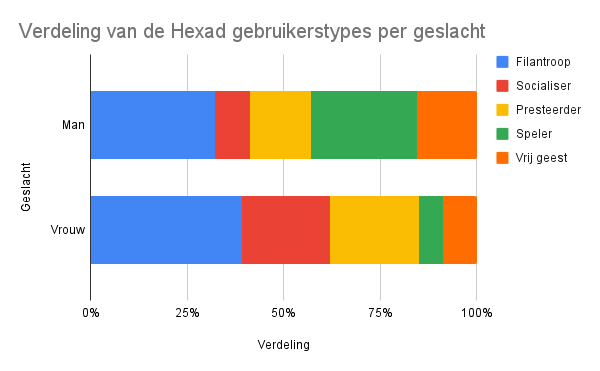
\includegraphics[width=\linewidth]{VerdelingGeslacht.png}
    \caption{Verdeling van de gebruikerstypes per geslacht.}
    \label{fig:verdelinggeslacht}
\end{figure}

\begin{table}
    \begin{center}
    \begin{tabular}{c|c|c|c|c}
        & Onderverdeling & $\chi^2$ & \textit{df} & \textit{p}     \\  
        \hline
        Individueel & Geslacht       & 7.76  & 4  & 0.101 \\
        & Leeftijd       & 18.67 & 24 & 0.770 \\ 
        \hline
        Hybride     & Geslacht       & 12.68 & 5  & 0.027 \\
        & Leeftijd       & 24.28 & 25 & 0.503 \\
    \end{tabular}
    \end{center}
\caption{Resultaten onafhankelijkheidstoets.}
\label{tab:onafhankelijkheidstoets}
\end{table}

In Figuur \ref{fig:verdelingleeftijd} is de verdeling van de gebruikerstypes bij elke leeftijdsgroep te zien. Hieruit blijkt dat hoe ouder een deelnemer is, hoe kleiner de kans is dat hij/zij een Speler is. De kans dat een deelnemer een Filantroop of Socialiser is neemt echter toe met de leeftijd. Met de onafhankelijkheidstoets werd nagegaan of een verband bestaat tussen de gebruikerstypes en de leeftijd. Tabel \ref{tab:onafhankelijkheidstoets} geeft weer dat voor $\chi^2$(24) = 18.67 bekomen werd en voor p = 0.770 bekomen werd.

\begin{figure}
    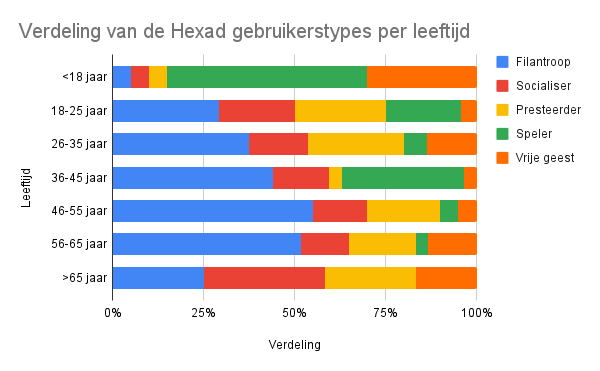
\includegraphics[width=\linewidth]{VerdelingLeeftijd.png}
    \caption{Verdeling van de gebruikerstypes per leeftijd.}
    \label{fig:verdelingleeftijd}
\end{figure}

Zoals eerder al werd vermeld kwam het soms voor dat bij het toewijzen van de gebruikerstypes gelijke scores werden behaald. Van alle deelnemers haalden 18.2\% van hen een gelijke score bij twee gebruikerstypes, 4.5\% haalde een gelijke score bij zowel drie gebruikerstypes als vier gebruikerstypes en 1.5\% haalden een gelijke score bij vijf gebruikerstypes. Geen enkele van de deelnemers haalde een gelijke score bij alle zes de types. Dit wil dus zeggen dat in totaal 28.7\% van de deelnemers geen specifiek gebruikerstype kreeg toegewezen. Het is daarom dat ook werd gekeken naar de verdeling van de zogenaamde hybride gebruikerstypes.

Bij het onderzoek naar de verdeling van de hybride gebruikerstypes werden zowel de gelijke scores bepaald als het verschil tussen de twee hoogste scores. Hieruit bleek dat voor 27.3\% van de deelnemers het verschil tussen de hoogste en tweede hoogste score 1 punt bedraagt, voor 22.7\% bedraagt het verschil 2 punten en voor 10.6\% bedraagt het verschil 3 punten. In combinatie met het aantal gelijke scores wil dit zeggen dat voor 89.3\% van de deelnemers het verschil tussen de hoogste scores ten hoogste 3 punten bedraagt. Dit is een laag verschil en toont aan dat gebruikers niet enkel door hun hoogste score een gebruikerstype kunnen worden toegewezen. In Tabel \ref{tab:aandeelhybridetypes} is daarom het aantal deelnemers te zien bij elke combinatie van toegewezen gebruikerstypes met een maximum verschil in scores van 3.

\begin{table}
    \begin{center}
        \begin{tabular}{c|c|c|c|c|c}
            \multicolumn{5}{c|}{\textbf{Gebruikerstypen}} & \textbf{Percentage} (\%)\\
            \hline
            Filantroop & Socialiser & & & & 16,7\% \\
            \hline
            Filantroop & Presteerder & & & & 16,7\%\\
            \hline
            Filantroop & Vrije geest & & & & 9,1\%\\
            \hline
            Presteerder & Speler & & & & 9,1\%\\
            \hline
            Presteerder & Socialiser & & & & 6,1\%\\
            \hline
            Speler & Vrije geest & & & & 4,5\%\\
            \hline
            Filantroop & Socialiser & Vrije geest & & & 4,5\%\\
            \hline
            Presteerder & Vrije geest & & & & 3,0\%\\
            \hline
            Socialiser & Vrije geest & & & & 3,0\%\\
            \hline
            Filantroop & Presteerder & Socialiser & & & 3,0\%\\
            \hline
            Filantroop & Speler & & & & 1,5\%\\
            \hline
            Filantroop & Socialiser & Speler & & & 1,5\%\\
            \hline
            Filantroop & Presteerder & Vrije geest & & & 1,5\%\\
            \hline
            Filantroop & Presteerder & Speler & & & 1,5\%\\
            \hline
            Presteerder & Speler & Vrije geest & & & 1,5\%\\
            \hline
            Filantroop & Socialiser & Speler & Vrije geest & & 1,5\%\\
            \hline
            Presteerder & Socialiser & Speler & Vrije geest & & 1,5\%\\
            \hline
            Filantroop & Presteerder & Socialiser & Vrije geest & & 1,5\%\\
            \hline
            Filantroop & Presteerder & Speler & Socialiser & Vrije geest & 1,5\%\\
        \end{tabular}
    \end{center}
    \caption{Aandeel van de hybride gebruikerstypes.}
    \label{tab:aandeelhybridetypes}
\end{table}

Figuur \ref{fig:hybridegeslacht} toont de verdeling van de zes meeste voorkomende hybride gebruikerstypes per geslacht. Bij de vrouwen is te zien dat ze bestaan uit een groter aandeel Filantroop-Presteerders en Filantroop-Socialisers. Bij de mannen zijn dan weer meer Presteerder-Spelers en Speler-Vrije geesten te vinden. Het Filantroop-Presteerder hybride gebruikerstype is bij de mannen niet te vinden. Met de onafhankelijkheidstoets werd nagegaan of een verband bestaat tussen de hybride gebruikerstypes en het geslacht. In Tabel \ref{tab:onafhankelijkheidstoets} is te zien dat voor $\chi^2$(5) = 12.68 bekomen werd en voor p = 0.027 bekomen werd.

\begin{figure}
    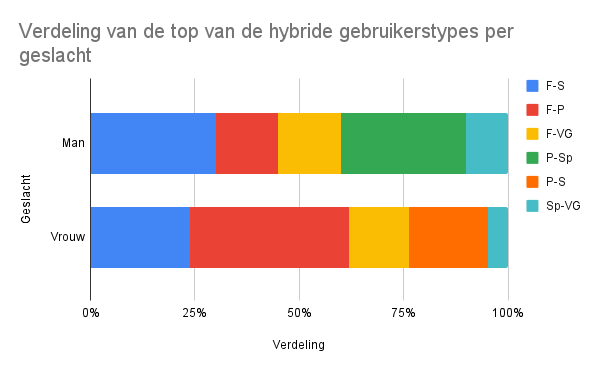
\includegraphics[width=\linewidth]{HybrideGeslacht.png}
    \caption{Verdeling van de top van de hybride gebruikerstypes per geslacht.}
    \label{fig:hybridegeslacht}
\end{figure}

In Figuur \ref{fig:hybrideleeftijd} is te zien dat het aandeel van de Filosoof-Socialisers en Filosoof-Presteerders met de leeftijd stijgt. Presteerder-Spelers en Speler-Vrije geesten zijn dan weer niet te vinden bij de oudere deelnemers. Aan de hand van de onafhankelijkheidstoets werd nagegaan of een verband bestaat tussen de hybride gebruikerstypes en de leeftijd. Tabel \ref{tab:onafhankelijkheidstoets} toont dat voor $\chi^2$(25) = 24,28 bekomen werd en voor p = 0.503 bekomen werd.

\begin{figure}
    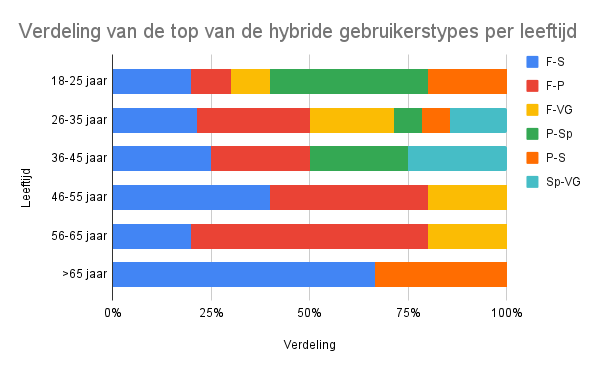
\includegraphics[width=\linewidth]{HybrideLeeftijd.png}
    \caption{Verdeling van de top van de hybride gebruikerstypes per leeftijd.}
    \label{fig:hybrideleeftijd}
\end{figure}

\textbf{Bespreking}

Figuur \ref{fig:vergelijkingonderzoek} toont een vergelijking tussen de verdeling van de steekproef uit het onderzoek van \textcite{Tondello2016} en de verdeling van de steekproef van dit onderzoek. Hierin is te zien dat er een verschil bestaat in de verdeling van de gebruikerstypes. In het onderzoek van \textcite{Tondello2016} zijn de Filantropen (24.0\%), de Presteerders (24.0\%) en de Vrij geesten (22.0\%) de dominante types terwijl in dit onderzoek de Filantropen (32.0\%), de Socialisers (20.6\%) en de Presteerders (20.6\%) het grootste aandeel vormen. Het grootste verschil met hun onderzoek is dat de Vrije geesten (11.3\%) maar een half zo groot aandeel vormen binnen dit onderzoek. Het Ontwrichter gebruikerstype ontbreekt aangezien geen enkele deelnemer dit type toegewezen gekregen heeft. Dit is vergelijkbaar met het onderzoek van Tondello et al. waar slechts 1.0\% als Ontwrichter gezien werd.

Uit de resultaten van de onafhankelijkheidstoets, te zien in Tabel \ref{tab:onafhankelijkheidstoets}, kan afgeleid worden dat tussen de individuele gebruikerstypes en het geslacht geen significante associatie bestaat. Ook tussen de individuele gebruikerstypes en de leeftijd kan geen significante associatie worden opgemaakt. Voor de hybride gebruikerstypes valt op dat de resultaten aangeven dat een associatie met het geslacht bestaat. Tussen de hybride gebruikerstypes en de leeftijd tonen de resultaten opnieuw dat geen associatie hiertussen bestaat. Deze resultaten kunnen echter als onbetrouwbaar worden beschouwd gezien de kleine steekproefgrootte en gelet op het feit dat niet aan de regel van Cochran is voldaan.

\subsection{Prototype}

Nadat de deelnemers werden onderverdeeld in verschillende gebruikerstypes op basis van hun antwoorden uit het tweede deel van de enquête, werden aan hen zeven stellingen voorgelegd. Zoals in Hoofdstuk~\ref{ch:methodologie} werd vermeld, zijn deze stellingen gebaseerd op de ervaring bij het gebruiken van het prototype. De deelnemers gaven bij deze stellingen aan of ze hiermee akkoord gingen of niet. Dit gebeurde aan de hand van een Likert-schaal van 5 punten (1 = helemaal niet akkoord, 2 = niet akkoord, 3 = neutraal, 4 = akkoord, 5 = volledig akkoord). Hieronder volgt een opsomming van de verschillende stellingen:

\begin{itemize}
    \item Stelling 1 (S1): \textit{Ik ben nu sneller bereid om meer enquêtes in te vullen.}
    \item Stelling 2 (S2): \textit{Ik wil meer enquêtes invullen om mijn aantal behaalde punten te verhogen.}
    \item Stelling 3 (S3): \textit{Ik ben nu sneller bereid om enquêtes tot het einde in te vullen omdat ik voor elke ingevulde pagina punten krijg.}
    \item Stelling 4 (S3): \textit{Ik wil meer enquêtes delen om mijn aantal behaalde punten te verhogen.}
    \item Stelling 5 (S5): \textit{Ik wil meer enquêtes invullen om mijn rangschikking op het leaderboard (scorebord) te verhogen.}
    \item Stelling 6 (S6): \textit{Ik wil meer enquêtes invullen om extra badges te behalen.}
    \item Stelling 7 (S7): \textit{Ik wil meer enquêtes invullen om beloningen te kunnen kopen in de rewardshop (beloningswinkel).}
\end{itemize}

\textbf{Resultaten}

Om te gaan bepalen of de gebruikersinteractie en -retentie wel degelijk verbeterd is, werd voor de individuele gebruikerstypes nagegaan wat hun respectievelijke scores zijn bij de verschillende stellingen. Voor de hybride gebruikerstypes werd ook nagegaan wat hun scores waren maar hier werd de analyse beperkt tot de vier grootste groepen van de hybride gebruikerstypes. De overige groepen hadden slechts een grootte van 3 of kleiner. In dit deel van het onderzoek werd gekozen om de scores niet verder onder te verdelen tussen geslacht of leeftijd. Deze beslissing werd genomen op basis van de resultaten van de onafhankelijkheidstoets uit het vorige deel, waar aangetoond werd dat geen significante associatie bestaat tussen de gebruikerstypes en het geslacht of de leeftijd.

De Figuren gaande van \ref{fig:s1} tot \ref{fig:s7_hybride} geven de resultaten weer per stelling. Tabel \ref{tab:mediaan} geeft de mediaan van de scores weer per gebruikerstype en per stelling.

\begin{table}
    \begin{center}
    \begin{tabular}{c|c|c|c|c|c|c|c|c}
        & Gebruikerstypes & S1 & S2 & S3  & S4  & S5  & S6 & S7  \\
        \hline
        Individueel & Filantroop             & 3  & 3  & 3   & 2   & 2   & 2  & 3   \\
        & Socialiser             & 3  & 3  & 3   & 3   & 2.5 & 3  & 4   \\
        & Vrije geest            & 3  & 3  & 3   & 2.5 & 2   & 2  & 4   \\
        & Presteerder            & 3  & 4  & 4   & 3   & 3   & 3  & 4   \\
        & Speler                 & 4  & 4  & 4   & 4   & 4   & 3  & 5   \\
        \hline
        Hybride     & Filantroop-Presteerder & 1  & 1  & 1   & 1   & 1   & 1  & 1   \\
        & Filantroop-Socialiser  & 3  & 3  & 3   & 2   & 2   & 2  & 3   \\
        & Filantroop-Vrije geest & 3  & 3  & 3   & 2.5 & 2   & 2  & 3.5 \\
        & Presteerder-Speler     & 4  & 5  & 4.5 & 4   & 4   & 4  & 5  
    \end{tabular}
    \end{center}
\caption{Mediaan van de scores bij elke stelling.}
\label{tab:mediaan}
\end{table}

\textbf{Stelling 1}

In Figuur \ref{fig:s1} is de verdeling van de scores voor de individuele gebruikerstypes van de eerste stelling te zien.  Bij deze stelling werd onderzocht of gebruikers nu meer bereid zijn om enquêtes te gaan invullen na de toevoeging van de game-design elementen aan het prototype In de figuur is te zien dat bijna 50\% van de Presteerders en meer dan 75\% van de Spelers na het gebruik van het prototype bereid zijn om meer enquêtes in te vullen.

\begin{figure}
    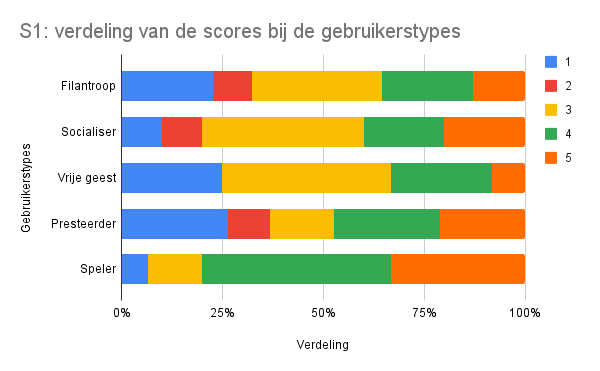
\includegraphics[width=\linewidth]{S1.png}
    \caption{Verdeling van de scores bij de individuele gebruikerstypes voor stelling 1.}
    \label{fig:s1}
\end{figure}

Figuur \ref{fig:s1_hybride} geeft de verdeling van de scores voor de hybride gebruikerstypes van de eerste stelling weer. Daarop is te zien dat geen enkele van de Presteerder-Spelers een score lager dan 4 aangaven, wat wil zeggen dat ze akkoord of volledig akkoord gingen met deze stelling. De meerderheid van de Filosoof-Presteerders gaf dan weer aan dat ze helemaal niet akkoord waren met deze stelling.

\begin{figure}
    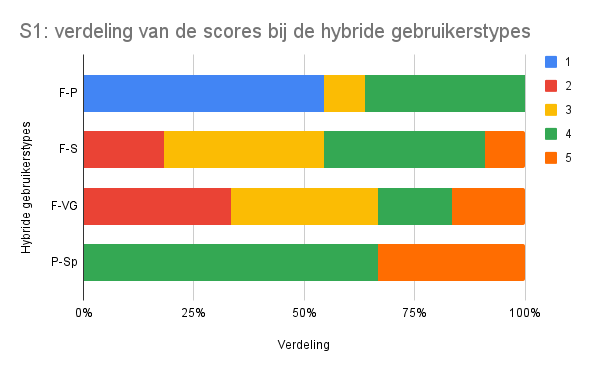
\includegraphics[width=\linewidth]{S1_Hybride.png}
    \caption{Verdeling van de scores bij de hybride gebruikerstypes voor stelling 1.}
    \label{fig:s1_hybride}
\end{figure}

Tabel \ref{tab:mediaan} geeft de mediaan van de scores weer. Daarop is te zien dat de scores van de Spelers en de Presteerder-Spelers een mediaan hebben van 4, wat wil zeggen dat de meerderheid van hen akkoord ging met deze stelling. De mediaan van de scores van de Filantroop-Presteerders toont dan weer dat het grootste deel van hen niet akkoord ging met deze stelling.

\textbf{Stelling 2}

De verdeling van de scores voor de individuele gebruikerstypes van de tweede stelling wordt weergegeven in Figuur \ref{fig:s2}. Hier werd onderzocht of de deelnemers na het gebruik van het prototype meer bereid zijn om enquêtes in te vullen om hun aantal verzamelde punten te verhogen. Meer dan 50\% van zowel de Presteerders als de Spelers gaven een hoge score aan wat wil zeggen dat ze met deze stelling akkoord of volledig akkoord zijn.

\begin{figure}
    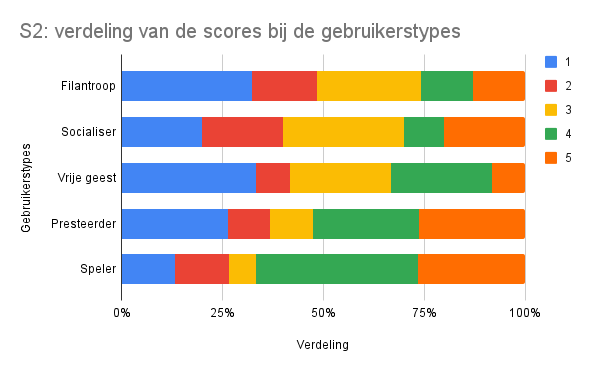
\includegraphics[width=\linewidth]{S2.png}
    \caption{Verdeling van de scores bij de individuele gebruikerstypes voor stelling 2.}
    \label{fig:s2}
\end{figure}

Voor de verdeling van de scores voor de hybride gebruikerstypes van de tweede stelling is te zien in Figuur \ref{fig:s2_hybride} dat de Presteerder-Spelers opnieuw akkoord of volledig akkoord gingen. Van alle Filosoof-Presteerders gaf de meerderheid weer aan dat ze niet akkoord gingen.

\begin{figure}
    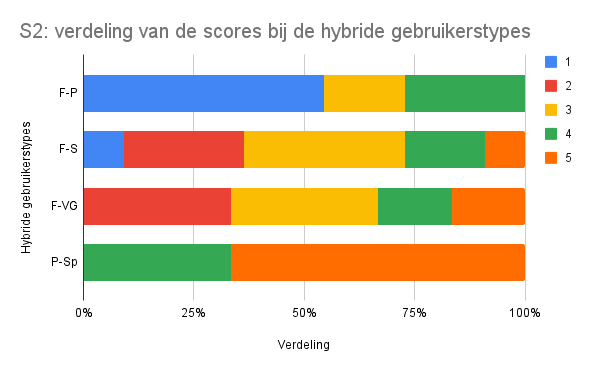
\includegraphics[width=\linewidth]{S2_Hybride.png}
    \caption{Verdeling van de scores bij de hybride gebruikerstypes voor stelling 2.}
    \label{fig:s2_hybride}
\end{figure}

De mediaan van de scores, te zien in tabel \ref{tab:mediaan}, toont dat het grootste deel van de Presteerders en Spelers akkoord ging met deze stelling. De mediaan van 5 bij de Presteerder-Spelers geeft weer dat de meeste van hen volledig akkoord gingen. Ook is opnieuw een mediaan van 1 te zien bij de Filantroop-Presteerders, wat wil zeggen dat het merendeel helemaal niet akkoord ging met deze stelling.

\textbf{Stelling 3}

Bij de derde stelling werd onderzocht of de deelnemers meer bereid zijn om enquêtes in te vullen omdat ze bij elke ingevulde pagina punten toegewezen krijgen. Figuur \ref{fig:s3} toont aan dat bijna 75\% van de Spelers hiermee akkoord gingen. Ook gaf meer dan 50\% van de Presteerders aan dat ze met deze stelling akkoord waren. Bijna de helft van de Filantropen was echter niet akkoord met deze stelling.

\begin{figure}
    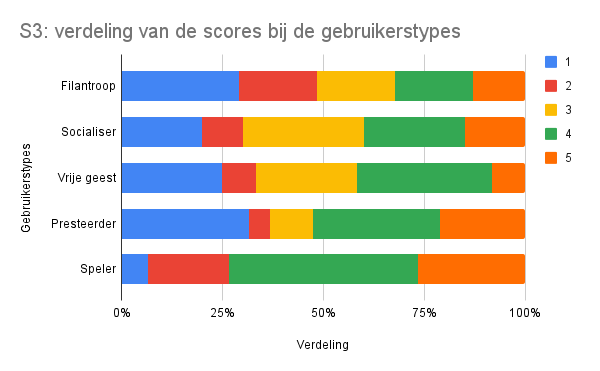
\includegraphics[width=\linewidth]{S3.png}
    \caption{Verdeling van de scores bij de individuele gebruikerstypes voor stelling 3.}
    \label{fig:s3}
\end{figure}

De scores van de hybride gebruikerstypes zijn te zien in Figuur \ref{fig:s3_hybride}. Net zoals de vorige stelling gaf geen enkele van de Presteerder-Spelers een score lager dan 4 aan. Ook gaf meer dan 50\% van de Filosoof-Presteerders opnieuw aan dat ze niet akkoord zijn met deze stelling.

\begin{figure}
    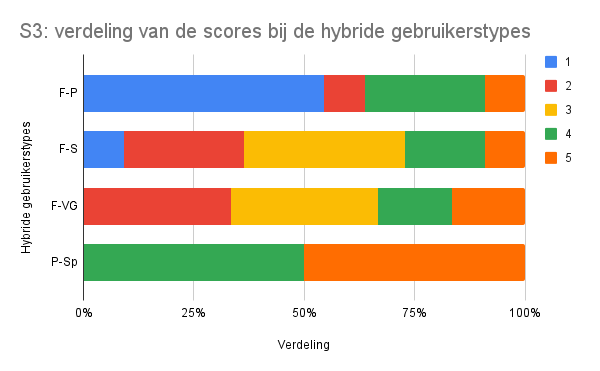
\includegraphics[width=\linewidth]{S3_Hybride.png}
    \caption{Verdeling van de scores bij de hybride gebruikerstypes voor stelling 3.}
    \label{fig:s3_hybride}
\end{figure}

Tabel \ref{tab:mediaan} toont opnieuw aan dat de meerderheid van de Presteerders, de Spelers en de Presteerder-Spelers akkoord ging met deze stelling, af te leiden uit de mediaan van 4 en 4.5. Voor de Filantroop-Presteerders zet dezelfde trend zich voort, waarbij een mediaan te zien is van 1. Dit wil dus zeggen dat ze opnieuw voor het grootste deel helemaal niet akkoord gingen met de stelling.

\textbf{Stelling 4}

In Figuur \ref{fig:s4} zijn de scores van de individuele gebruikerstypes voor stelling 4 te zien. Hierbij werd onderzocht of de deelnemers meer bereid zijn om enquêtes te gaan delen om punten te verzamelen. Uit de figuur is opnieuw op te maken dat meer dan 50\% van de Spelers aangaven dat ze met deze stelling akkoord gingen. Bij de verdeling van de scores van de Presteerders is een lichte daling te merken in vergelijking met de vorige stelling waardoor het aantal dat met deze stelling akkoord ging daalt tot net iets onder 50\%.

\begin{figure}
    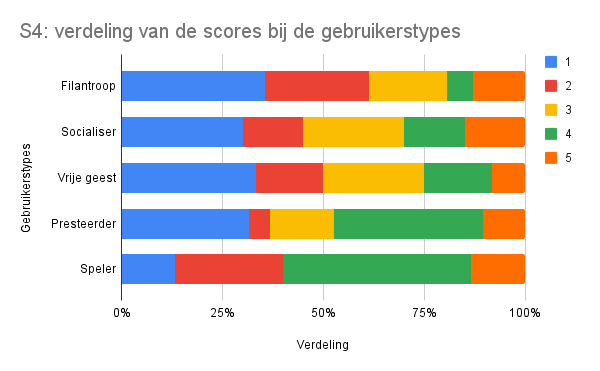
\includegraphics[width=\linewidth]{S4.png}
    \caption{Verdeling van de scores bij de individuele gebruikerstypes voor stelling 4.}
    \label{fig:s4}
\end{figure}

Figuur \ref{fig:s4_hybride} toont de scores bij stelling 4 voor de hybride gebruikerstypes. Hierbij valt sterk op dat alle Presteerder-Spelers een score van 4 aangaven wat wil zeggen dat ze akkoord gingen met de stelling maar niet volledig. Voor de overige hybride gebruikerstypes gaf 50\% of meer aan dat ze niet akkoord gingen met deze stelling.

\begin{figure}
    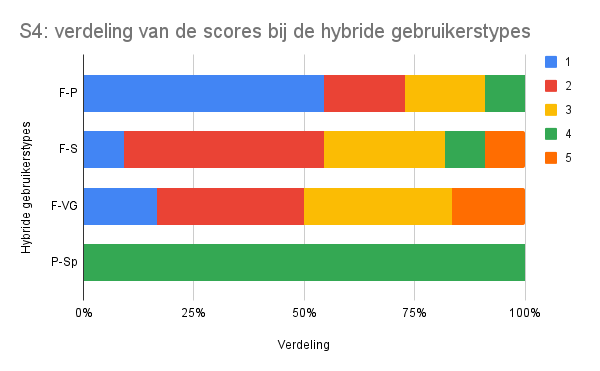
\includegraphics[width=\linewidth]{S4_Hybride.png}
    \caption{Verdeling van de scores bij de hybride gebruikerstypes voor stelling 4.}
    \label{fig:s4_hybride}
\end{figure}

De mediaan van de scores (Tabel \ref{tab:mediaan}) voor de Spelers en Presteerder-Spelers bedraagt 4, wat voor de Presteerder-Spelers een lichte daling is. Echter blijven ze nog steeds grotendeels akkoord met deze stelling, net zoals de Spelers. Voor de Filantropen, de Vrije geesten, de Presteerders, de Filantroop-Presteerders, de Filantroop-Socialisers en de Filantroop-Vrije geesten is ook een daling merkbaar. Dit wil zeggen dat, in vergelijking met de vorige stelling, een groter deel niet akkoord is met deze stelling. Voor de Filantroop-Presteerders blijft, net zoals alle vorige stellingen, de mediaan 1.

\textbf{Stelling 5}

Stelling 5 onderzocht of de deelnemers bereid zijn om meer enquêtes in te vullen om hun rangschikking op het scorebord te verhogen. In Figuur \ref{fig:s5} is te zien dat meer dan 50\% van de Spelers en net geen 50\% van de Presteerders aangaven dat ze met deze stelling akkoord gingen. Bij de Socialisers gaf 50\% aan dat ze niet met deze stelling akkoord gingen net zoals de meerderheid van de Filantropen en de Vrije geesten.

\begin{figure}
    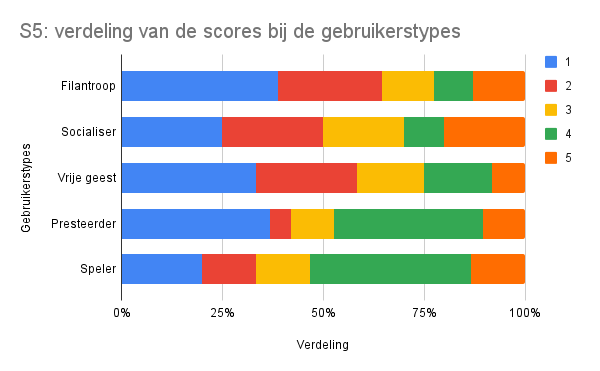
\includegraphics[width=\linewidth]{S5.png}
    \caption{Verdeling van de scores bij de individuele gebruikerstypes voor stelling 5.}
    \label{fig:s5}
\end{figure}

Figuur \ref{fig:s5_hybride} geeft voor de hybride gebruikerstypes weer dat, in tegenstelling tot de vorige stellingen, niet alle Presteerder-Spelers akkoord gingen met deze stelling. Bij de Filantroop-Socialisers en Filantroop-Vrij geesten gaf meer dan 50\% aan dat ze niet akkoord gingen met de stelling. Bijna alle Filantroop-Presteerders gingen niet akkoord met de stelling.

\begin{figure}
    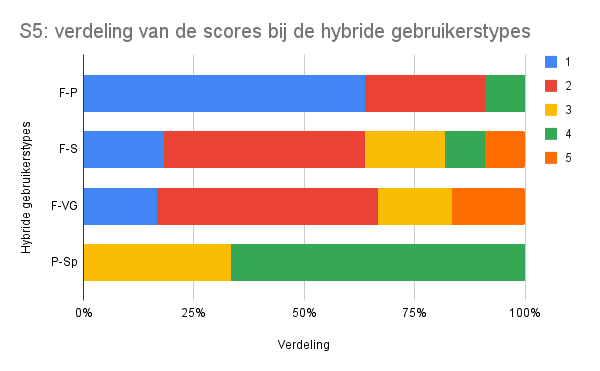
\includegraphics[width=\linewidth]{S5_Hybride.png}
    \caption{Verdeling van de scores bij de hybride gebruikerstypes voor stelling 5.}
    \label{fig:s5_hybride}
\end{figure}

In Tabel \ref{tab:mediaan} is een mediaan van 4 voor zowel de Spelers als de Presteerder-Spelers te zien, waardoor opnieuw kan afgeleid worden dat de meerderheid van hen akkoord gaat met deze stelling. Voor de Filantropen, Socialisers, Vrije geesten en de overige hybride gebruikerstypes is een mediaan te zien van 2.5 of lager. Dit wil zeggen dat de helft of meer van hen niet akkoord ging met de vijfde stelling.

\textbf{Stelling 6}

Om de invloed van de badges binnen het prototype te onderzoeken werd aan de deelnemers gevraagd of ze bereid zijn meer enquêtes in te vullen om badges te behalen. Figuur \ref{fig:s6} toont aan dat voor de eerste maal minder dan 50\% van de Spelers met deze stelling akkoord ging. De meerderheid van de Filantropen en Vrije geesten ging niet akkoord met deze stelling.

\begin{figure}
    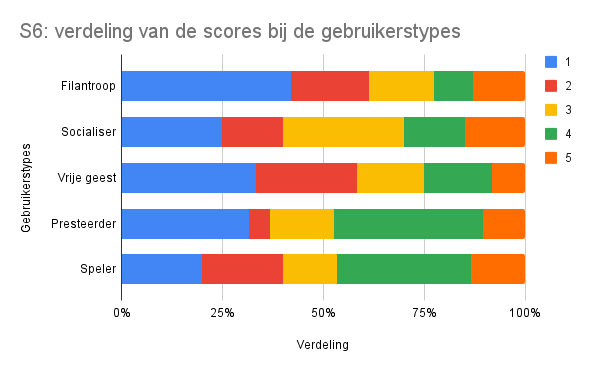
\includegraphics[width=\linewidth]{S6.png}
    \caption{Verdeling van de scores bij de individuele gebruikerstypes voor stelling 6.}
    \label{fig:s6}
\end{figure}

Bij de hybride gebruikerstypes, waarvan de score te zien is in Figuur \ref{fig:s6_hybride}, is dezelfde verdeling van de scores te zien voor de Presteerder-Spelers als bij de vorige stelling. Daaruit is af te leiden dat opnieuw niet alle Presteerder-Spelers akkoord gingen met deze stelling. Ook gaf meer dan 50\% van de Filantroop-Socialisers en de Filantroop-Vrije geesten opnieuw aan dat ze niet akkoord gingen met deze stelling. Voor de Filantroop-Presteerders is het aantal dat niet akkoord ging met de stelling iets gedaald in vergelijking met de vorige stelling maar nog steeds hoger dan 50\%.

\begin{figure}
    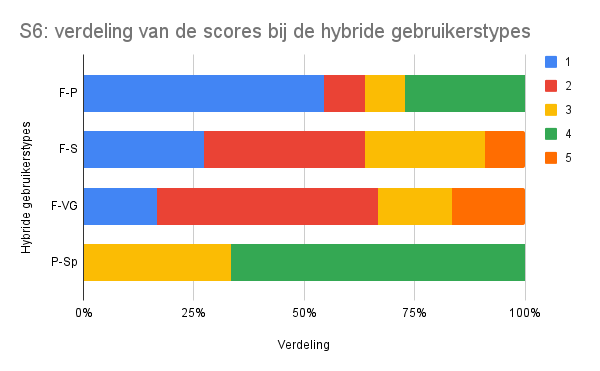
\includegraphics[width=\linewidth]{S6_Hybride.png}
    \caption{Verdeling van de scores bij de hybride gebruikerstypes voor stelling 6.}
    \label{fig:s6_hybride}
\end{figure}

Tabel \ref{tab:mediaan} toont dat voor de Spelers de mediaan van hun scores voor de eerste en enige maal lager dan 4 bedraagt, wat erop wijst dat minder dan de helft akkoord ging met deze stelling. De Presteerder-Spelers blijven een mediaan behouden van 4 wat erop wijst dat de meerderheid akkoord ging. Voor de overige gebruikerstypes blijft dezelfde mediaan behouden in vergelijking met de vorige stelling maar met één uitzondering, de Socialisers. Bij hen is de mediaan met een half punt gestegen wat wil zeggen dat het deel dat niet akkoord ging gedaald is.

\textbf{Stelling 7}

Bij de zevende en laatste stelling werd de invloed van de beloningswinkel onderzocht. Aan de deelnemers werd gevraagd of ze meer bereid zijn om enquêtes in te vullen om beloningen te kunnen aanschaffen. In Figuur \ref{fig:s7} is te zien dat de deelnemers over het algemeen het meeste akkoord waren met deze stelling. Meer dan 50\% van de Socialisers, Vrije geesten, Presteerders en Spelers gaf aan dat ze met deze stelling akkoord gingen. Enkel bij de Filantropen was het aantal lager dan 50\%.

\begin{figure}
    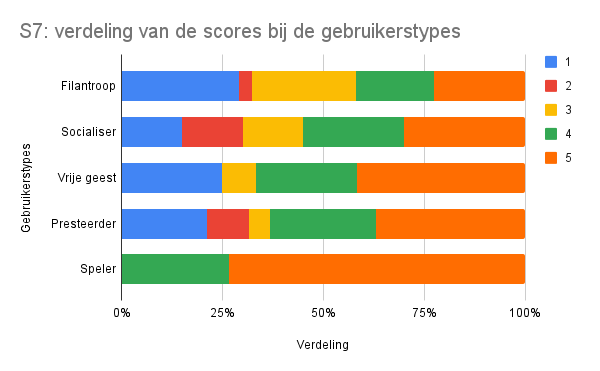
\includegraphics[width=\linewidth]{S7.png}
    \caption{Verdeling van de scores bij de individuele gebruikerstypes voor stelling 7.}
    \label{fig:s7}
\end{figure}

Figuur \ref{fig:s7_hybride} geeft weer dat bij de scores van de hybride gebruikerstypes de Presteerder-Spelers allemaal akkoord gingen met de stelling, meer dan 75\% was zelfs volledig akkoord. Voor de Filantroop-Vrij geesten was 50\% akkoord. De meerderheid van de Filantroop-Presteerders ging niet akkoord met de stelling.

\begin{figure}
    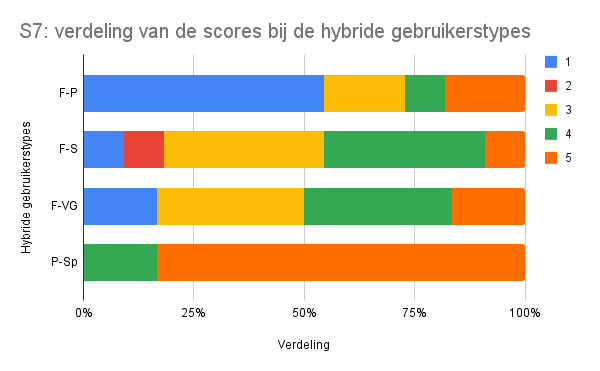
\includegraphics[width=\linewidth]{S7_Hybride.png}
    \caption{Verdeling van de scores bij de hybride gebruikerstypes voor stelling 7.}
    \label{fig:s7_hybride}
\end{figure}

Tabel \ref{tab:mediaan} toont aan dat de mediaan voor bijna alle gebruikerstypes de hoogste waarde heeft, met zelfs een mediaan van 5 voor zowel de Spelers als de Presteerder-Spelers. Dit wil zeggen dat voor bijna alle types het grootste deel akkoord ging met de laatste stelling. Enkel bij de Filantropen, de Filantroop-Presteerders en de Filantroop-Socialisers blijft het aandeel dat akkoord ging kleiner dan de helft. Voor de Filantroop-Presteerders is geen verandering merkbaar met vorige stellingen. De mediaan van 1 blijft behouden wat opnieuw wil zeggen dat het grootste deel niet akkoord ging met deze stelling.

\textbf{Bespreking}

Uit de weergave van de resultaten voor de individuele gebruikerstypes valt af te leiden dat meer dan 50\% van de Spelers met bijna elke stelling akkoord of zelfs volledig akkoord gingen. Deze stellingen waren van toepassing op het puntensysteem, badgesysteem en scorebord die binnen het prototype werden ontwikkeld. Aan de hand van deze resultaten valt dus af te leiden dat Spelers vooral door punten, badges en scoreborden worden gemotiveerd. In de onderzoeken van zowel \textcite{Tondello2016} als \textcite{Carreno2018} blijkt dat Spelers het sterkst gemotiveerd worden door extrinsieke beloningen, waardoor de ontwerpelementen die het beste passen bij Spelers punten, scoreborden en badges zijn. Deze resultaten werden bevestigd door dit onderzoek.

Opvallend is dat voor stelling 6 minder dan 50\% van de Spelers akkoord gingen. Dit kan echter verklaard worden door technische problemen met het weergeven van de badge. Als noodoplossing werd gekozen om een afbeelding te nemen van het verkrijgen van een badge en dit voor te leggen aan de deelnemers. Dit bereikte echter niet het gewenste psychologische effect van het verdienen van een badge waardoor de resultaten lager zijn dan verwacht.





% Voeg hier je eigen hoofdstukken toe die de ``corpus'' van je bachelorproef
% vormen. De structuur en titels hangen af van je eigen onderzoek. Je kan bv.
% elke fase in je onderzoek in een apart hoofdstuk bespreken.

%\input{...}
%\input{...}
%...

%%=============================================================================
%% Conclusie
%%=============================================================================

\chapter{Conclusie}
\label{ch:conclusie}

% TODO: Trek een duidelijke conclusie, in de vorm van een antwoord op de
% onderzoeksvra(a)g(en). Wat was jouw bijdrage aan het onderzoeksdomein en
% hoe biedt dit meerwaarde aan het vakgebied/doelgroep? 
% Reflecteer kritisch over het resultaat. In Engelse teksten wordt deze sectie
% ``Discussion'' genoemd. Had je deze uitkomst verwacht? Zijn er zaken die nog
% niet duidelijk zijn?
% Heeft het onderzoek geleid tot nieuwe vragen die uitnodigen tot verder 
%onderzoek?

Tijdens dit onderzoek werd onderzocht hoe gamification kan worden geïmplementeerd en wat het effect hiervan is op de gebruikersinteractie en -retentie. Om dit te onderzoeken werd op de volgende onderzoeksvragen een antwoord gegeven:

\begin{itemize}
    \item Op welke verschillende manieren kan gamification worden geïmplementeerd?
    \item Welke stappen zijn nodig om gamification toe te voegen aan een reeds bestaand platform?
    \item Vergroot het toevoegen van gamification de gebruikersinteractie en -retentie?
\end{itemize}

Hiervoor werd een prototype uitgewerkt waarbinnen enkele ontwerpelementen van gamification werden toegevoegd. Op basis van dit prototype werd tevens een gebruikersonderzoek gevoerd.

Om de eerste onderzoeksvraag te kunnen beantwoorden werd onderzoek gedaan naar de verschillende ontwerpelementen binnen gamification. Dit deel van het onderzoek werd uitgevoerd in de literatuurstudie in Hoofdstuk~\ref{ch:stand-van-zaken}. Hieruit werd duidelijk dat gamification een aantal veelvoorkomende ontwerpelementen omvat waaronder: punten, badges, scoreborden, prestatiegrafieken, betekenisvolle verhalen, avatars en teamleden. Deze elementen worden het vaakst geïmplementeerd omdat ze direct zichtbaar zijn voor de spelers, gemakkelijk geactiveerd of gedeactiveerd worden en omdat ze spelers sterk motiveren. Voor de spelontwerpers zijn ze gemakkelijk te implementeren omdat ze deel uitmaken van het zichtbare deel en niet afhankelijk zijn van onderliggende mechanismen.

De tweede onderzoeksvraag onderzocht welke stappen nodig zijn om gamification toe te voegen aan een reeds bestaand platform. Zoals eerder vermeld werd een prototype uitgewerkt, op basis van het platform Innerdreams, waaraan een aantal ontwerpelementen werden toegevoegd: punten, badges, een scorebord en een beloningswinkel. Na het uitwerken van het prototype is duidelijk geworden dat het toevoegen van deze ontwerpelementen geen fundamentele veranderingen vereisten aan het bestaande systeem. De enige benodigde verandering was het aanpassen van de bestaande gebruikerstabel zodat deze de verzamelde punten kon bijhouden. Alle overige toevoegingen werden ingewerkt binnen het bestaande systeem zonder aan de reeds bestaande functionaliteiten te raken.

De derde en laatste onderzoekvraag onderzocht of het toevoegen van gamification de gebruikersinteractie en -retentie vergroot. Zoals reeds vermeld werd op basis van het prototype een gebruikersonderzoek gevoerd. Uit de resultaten van dit onderzoek blijkt dat de gebruikersinteractie en -retentie wel degelijk vergroot wordt maar dat dit sterk afhankelijk is van het gebruikerstype. Het is daarom dat het noodzakelijk is om een gebruikersonderzoek te voeren als men ervoor kiest om gamification te gaan implementeren. Zo een gebruikersonderzoek is nodig om te kunnen bepalen uit welke soorten van gebruikerstypes de huidige of toekomstige gebruikers bestaan. Het is bij dit onderzoek ook belangrijk om te onthouden dat een gebruiker vaak niet één gebruikerstype heeft maar door meerdere types kan beschreven worden. Op basis van dit gebruikersonderzoek kan dan bepaald worden welke ontwerpelementen geïmplementeerd moeten worden en op welke manier ze moeten worden aangepast.

Aangezien het gebruikersonderzoek werd uitvoerd op een kleine steekproefgrootte (N = 66) kon niet worden bepaald of een associatie bestond tussen de verschillende gebruikerstypes en het geslacht of de leeftijden. Hierdoor werd bij het onderzoeken of gamification de gebruikersinteractie en -retentie verbeterd geen verder onderscheid gemaakt tussen geslacht of leeftijd. Een soortgelijk onderzoek met een grotere steekproefgrootte en een gelijkere verdeling zou hierover duidelijkheid kunnen scheppen.




%%=============================================================================
%% Bijlagen
%%=============================================================================

\appendix
\renewcommand{\chaptername}{Appendix}

%%---------- Onderzoeksvoorstel -----------------------------------------------

\chapter{Onderzoeksvoorstel}

Het onderwerp van deze bachelorproef is gebaseerd op een onderzoeksvoorstel dat vooraf werd beoordeeld door de promotor. Dat voorstel is opgenomen in deze bijlage.

% Verwijzing naar het bestand met de inhoud van het onderzoeksvoorstel
%---------- Inleiding ---------------------------------------------------------

\section{Introductie} % The \section*{} command stops section numbering
\label{sec:introductie}

Hier introduceer je werk. Je hoeft hier nog niet te technisch te gaan.

Je beschrijft zeker:

\begin{itemize}
  \item de probleemstelling en context
  \item de motivatie en relevantie voor het onderzoek
  \item de doelstelling en onderzoeksvraag/-vragen
\end{itemize}

%---------- Stand van zaken ---------------------------------------------------

\section{State-of-the-art}
\label{sec:state-of-the-art}

Hier beschrijf je de \emph{state-of-the-art} rondom je gekozen onderzoeksdomein. Dit kan bijvoorbeeld een literatuurstudie zijn. Je mag de titel van deze sectie ook aanpassen (literatuurstudie, stand van zaken, enz.). Zijn er al gelijkaardige onderzoeken gevoerd? Wat concluderen ze? Wat is het verschil met jouw onderzoek? Wat is de relevantie met jouw onderzoek?

Verwijs bij elke introductie van een term of bewering over het domein naar de vakliteratuur, bijvoorbeeld~\autocite{Doll1954}! Denk zeker goed na welke werken je refereert en waarom.

% Voor literatuurverwijzingen zijn er twee belangrijke commando's:
% \autocite{KEY} => (Auteur, jaartal) Gebruik dit als de naam van de auteur
%   geen onderdeel is van de zin.
% \textcite{KEY} => Auteur (jaartal)  Gebruik dit als de auteursnaam wel een
%   functie heeft in de zin (bv. ``Uit onderzoek door Doll & Hill (1954) bleek
%   ...'')

Je mag gerust gebruik maken van subsecties in dit onderdeel.

%---------- Methodologie ------------------------------------------------------
\section{Methodologie}
\label{sec:methodologie}

Hier beschrijf je hoe je van plan bent het onderzoek te voeren. Welke onderzoekstechniek ga je toepassen om elk van je onderzoeksvragen te beantwoorden? Gebruik je hiervoor experimenten, vragenlijsten, simulaties? Je beschrijft ook al welke tools je denkt hiervoor te gebruiken of te ontwikkelen.

%---------- Verwachte resultaten ----------------------------------------------
\section{Verwachte resultaten}
\label{sec:verwachte_resultaten}

Hier beschrijf je welke resultaten je verwacht. Als je metingen en simulaties uitvoert, kan je hier al mock-ups maken van de grafieken samen met de verwachte conclusies. Benoem zeker al je assen en de stukken van de grafiek die je gaat gebruiken. Dit zorgt ervoor dat je concreet weet hoe je je data gaat moeten structureren.

%---------- Verwachte conclusies ----------------------------------------------
\section{Verwachte conclusies}
\label{sec:verwachte_conclusies}

Hier beschrijf je wat je verwacht uit je onderzoek, met de motivatie waarom. Het is \textbf{niet} erg indien uit je onderzoek andere resultaten en conclusies vloeien dan dat je hier beschrijft: het is dan juist interessant om te onderzoeken waarom jouw hypothesen niet overeenkomen met de resultaten.



%%---------- Andere bijlagen --------------------------------------------------
% TODO: Voeg hier eventuele andere bijlagen toe
%\input{...}

%%---------- Referentielijst --------------------------------------------------

\printbibliography[heading=bibintoc]

\end{document}
